\documentclass[12pt,a4paper]{report}
\usepackage{fontspec}
\usepackage[french]{babel}
\usepackage{graphicx}
\usepackage{geometry}
\usepackage{titlesec}
\usepackage{tocloft}
\usepackage{hyperref}
\usepackage{xcolor}
\usepackage{fancyhdr}
\usepackage{setspace}
\usepackage{lipsum}
\usepackage{enumitem}
\usepackage{float}
\usepackage{caption}
\usepackage{longtable}
\usepackage{booktabs}
\usepackage{listings}
\usepackage{colortbl}
\usepackage{amssymb}
\usepackage{pdfpages}

% Set fonts for XeLaTeX
\setmainfont{DejaVu Serif}
\setmonofont{DejaVu Sans Mono}

% Geometry
\geometry{
    top=1.5cm,
    bottom=2.5cm,
    left=3cm,
    right=2.5cm
}

% Colors
\definecolor{supnumgreen}{RGB}{27,107,47}
\definecolor{supnumyellow}{RGB}{245,197,24}
\definecolor{headingcolor}{RGB}{27,107,47}
\definecolor{codebg}{RGB}{245,245,245}
\definecolor{okgreen}{RGB}{0,150,0}

% Hyperlinks
\hypersetup{
    colorlinks=true,
    linkcolor=supnumgreen,
    urlcolor=blue,
    citecolor=supnumgreen
}

% Header/Footer
\pagestyle{fancy}
\fancyhf{}
\fancyhead[L]{\small Baligh -- Rapport de Projet}
\fancyhead[R]{\small SUPNUM}
\fancyfoot[C]{\thepage}
\setlength{\headheight}{14pt}
\renewcommand{\headrulewidth}{0.4pt}
\renewcommand{\footrulewidth}{0.4pt}

% Chapter headings
\titleformat{\chapter}[display]
  {\normalfont\Huge\bfseries\color{supnumgreen}}
  {\chaptertitlename\ \thechapter}{20pt}{\Huge}
\titlespacing*{\chapter}{0pt}{50pt}{40pt}

\titleformat{\section}
  {\normalfont\Large\bfseries\color{supnumgreen}}
  {\thesection}{1em}{}

\titleformat{\subsection}
  {\normalfont\large\bfseries\color{supnumgreen!80!black}}
  {\thesubsection}{1em}{}

% Table of contents styling
\renewcommand{\cftchapfont}{\bfseries\color{supnumgreen}}
\renewcommand{\cftsecfont}{\color{black}}
\renewcommand{\cftsubsecfont}{\color{black!70}}

% Remove "Chapter" prefix from TOC
\renewcommand{\cftchappresnum}{}
\renewcommand{\cftchapaftersnum}{}

% Line spacing
\setstretch{1.5}

% Caption styling
\captionsetup{labelfont={bf,color=supnumgreen},font=small}

% Checkmark command
\newcommand{\done}{\textcolor{okgreen}{\checkmark}}

% Code listing style
\lstdefinestyle{codeblock}{
    backgroundcolor=\color{codebg},
    basicstyle=\ttfamily\small,
    keywordstyle=\color{blue}\bfseries,
    stringstyle=\color{red},
    commentstyle=\color{green!50!black},
    numbers=left,
    numberstyle=\tiny,
    frame=single,
    breaklines=true,
    tabsize=2,
    showstringspaces=false
}

% Command for screenshot inclusion
\newcommand{\screenshot}[3][0.45]{%
    \begin{figure}[H]
        \centering
        \includegraphics[width=#1\textwidth]{#2}
        \caption{#3}
        \label{fig:#2}
    \end{figure}
}

\begin{document}

% =====================================================
% PAGE DE GARDE
% =====================================================
\begin{titlepage}
    \centering
    \vspace*{1cm}

    
\includegraphics[width=4cm]{captures-application/supnum-logo.jpeg}\\[0.5cm]

    \textbf{\Large Institut Supérieur du Numérique}\\[0.3cm]
    \textbf{SUPNUM -- Mauritanie}\\[1cm]

    \rule{\textwidth}{1.5pt}\\[0.3cm]

    {\Huge \textbf{Baligh}}\\[0.3cm]
    {\Large \textbf{Application Mobile de Signalement Citoyen}}\\[0.2cm]
    {\large Projet de Développement Mobile --- Flutter}\\[0.3cm]

    \rule{\textwidth}{1.5pt}\\[1cm]

    \textbf{Réalisé par :}\\[0.3cm]
    \begin{tabular}{ll}
        \textbf{Abdy Mohameden} & 24068\\
        \textbf{Abdselam Abdelvetah} & 24139\\
        \textbf{Hassen Oumeiry} & 24238\\
        \textbf{Ahmedou Bedou} & 24157\\
    \end{tabular}\\[0.5cm]

    \textbf{Encadré par :}\\[0.2cm]
    \textit{Équipe pédagogique SUPNUM}\\[0.5cm]

    \vfill
    \textbf{13 juin 2026}
\end{titlepage}

% =====================================================
% RÉSUMÉ
% =====================================================
\chapter*{Résumé}
\thispagestyle{plain}
\addcontentsline{toc}{chapter}{Résumé}

\textbf{Baligh} (« Signaler » en arabe) est une application mobile de signalement citoyen développée dans le cadre du projet de Développement Mobile de l'Institut Supérieur du Numérique (SUPNUM). Elle permet aux citoyens mauritaniens de signaler des problèmes locaux (infrastructures endommagées, risques environnementaux, préoccupations sécuritaires, etc.), de consulter les signalements des autres utilisateurs, de vérifier la crédibilité des rapports via un système de vote, et de communiquer directement avec les auteurs des signalements.

L'application est construite avec \textbf{Flutter} (Dart), suivant une architecture \textbf{MVC} (Modèle-Vue-Contrôleur) avec \textbf{Provider} pour la gestion d'état. Le backend est assuré par \textbf{Supabase} (PostgreSQL, Auth, Storage, Realtime). Trois langues sont supportées : arabe (RTL), français et anglais. L'application utilise \textbf{OpenStreetMap} via \texttt{flutter\_map} avec mise en cache des tuiles pour la cartographie interactive.

Ce rapport présente l'analyse, la conception, les technologies utilisées et l'ensemble des fonctionnalités développées dans le cadre de ce projet.

\vspace{0.5cm}
\textbf{Mots-clés :} Flutter, Dart, Application mobile, Signalement citoyen, MVC, Provider, Supabase, OpenStreetMap, Mauritanie, Internationalisation.

% =====================================================
% TABLE DES MATIÈRES
% =====================================================
\tableofcontents
\newpage

% =====================================================
% TABLE DES FIGURES
% =====================================================
\listoffigures
\newpage

% =====================================================
% INTRODUCTION
% =====================================================
\chapter*{Introduction générale}
\thispagestyle{plain}
\addcontentsline{toc}{chapter}{Introduction générale}

La Mauritanie, comme de nombreux pays en développement, fait face à des défis importants en matière de gestion des infrastructures urbaines et de communication entre les citoyens et les autorités. Les problèmes tels que les nids-de-poule, les lampadaires défectueux, les décharges sauvages ou les risques sécuritaires sont souvent signalés de manière informelle, sans suivi structuré.

Dans ce contexte, le présent projet vise à développer une application mobile de signalement citoyen nommée \textbf{Baligh}, permettant aux citoyens de signaler facilement des problèmes, d'en suivre l'évolution et de contribuer à la vie citoyenne de manière transparente et collaborative.

Ce rapport est structuré en six chapitres :
\begin{enumerate}
    \item \textbf{Présentation du projet} -- Objectifs, cahier des charges et organisation de l'équipe.
    \item \textbf{Contexte} -- Contexte institutionnel et social du projet.
    \item \textbf{Analyse des besoins} -- Besoins fonctionnels et non fonctionnels.
    \item \textbf{Conception et méthodologie} -- Architecture, technologies et méthodologie de travail.
    \item \textbf{Fonctionnalités développées} -- Présentation détaillée de chaque fonctionnalité avec captures d'écran.
    \item \textbf{Conclusion} -- Bilan du projet, difficultés rencontrées et perspectives.
\end{enumerate}

% =====================================================
% CHAPITRE 1 : PRÉSENTATION DU PROJET
% =====================================================
\chapter{Présentation du projet}

\section{Contexte et objectifs}

Baligh est une application de \textbf{signalement citoyen} destinée au contexte mauritanien. Elle permet à tout citoyen équipé d'un smartphone de :
\begin{itemize}
    \item Signaler un problème (infrastructure, environnement, sécurité, etc.) en quelques étapes simples ;
    \item Visualiser les signalements des autres citoyens sur une carte interactive ;
    \item Voter pour la crédibilité des signalements (confirmer ou infirmer) ;
    \item Communiquer avec les auteurs des signalements via une messagerie intégrée ;
    \item Recevoir des notifications sur les nouveaux signalements.
\end{itemize}

\section{Objectifs pédagogiques}

Ce projet s'inscrit dans le cadre du module de \textbf{Développement Mobile} de SUPNUM. Les objectifs pédagogiques sont :
\begin{itemize}
    \item Maîtriser le framework Flutter et le langage Dart ;
    \item Mettre en œuvre une architecture MVC avec gestion d'état via Provider ;
    \item Intégrer une base de données distante et une API (Supabase) ;
    \item Implémenter l'internationalisation (i18n) avec support multilingue ;
    \item Développer une interface utilisateur interactive et réactive ;
    \item Appliquer les bonnes pratiques de développement mobile.
\end{itemize}

\section{Cahier des charges}

Le cahier des charges, défini par l'équipe pédagogique, impose les contraintes suivantes :
\begin{itemize}
    \item Travail en groupe avec participation active de tous les membres ;
    \item Fonctionnalités interactives : formulaires, navigation multi-écrans, boutons d'action, CRUD ;
    \item Gestion d'état avec \textbf{Provider} ;
    \item Architecture \textbf{MVC} (Modèle-Vue-Contrôleur) ;
    \item Connexion à une \textbf{base de données} et à une \textbf{API} ;
    \item \textbf{Internationalisation} (au moins deux langues) ;
    \item Code clair, structuré et maintenable ;
    \item Projet original démontrant les compétences acquises.
\end{itemize}

\section{Organisation de l'équipe}

Le projet a été réalisé par une équipe de quatre étudiants, avec la répartition suivante des responsabilités :

\begin{table}[H]
    \centering
    \begin{tabular}{|c|l|l|}
        \hline
        \rowcolor{supnumgreen!20}
        \textbf{Étudiant} & \textbf{Matricule} & \textbf{Rôles principaux} \\
        \hline
        Abdy Mohameden & 24068 & Backend Supabase, DAOs, services, déploiement \\
        \hline
        Abdselam Abdelvetah & 24139 & UI/UX, cartographie, internationalisation \\
        \hline
        Hassen Oumeiry & 24238 & Gestion d'état (Provider), contrôleurs \\
        \hline
        Ahmedou Bedou & 24157 & Développement des fonctionnalités de vote,\\ 
        & & messagerie et notifications \\
        \hline
    \end{tabular}
    \caption{Répartition des tâches}
    \label{tab:team}
\end{table}

% =====================================================
% CHAPITRE 2 : CONTEXTE
% =====================================================
\chapter{Contexte}

\section{Contexte institutionnel}

L'\textbf{Institut Supérieur du Numérique (SUPNUM)} est un établissement d'enseignement supérieur mauritanien spécialisé dans les technologies de l'information et de la communication. Dans le cadre de sa formation en Développement Mobile, les étudiants sont amenés à réaliser un projet complet de conception et de développement d'une application mobile.

\section{Contexte social et environnemental}

En Mauritanie, les problèmes urbains sont fréquents et diversifiés :
\begin{itemize}
    \item Infrastructures routières dégradées (nids-de-poule, routes non bitumées) ;
    \item Problèmes d'éclairage public (lampadaires défectueux) ;
    \item Assainissement et gestion des déchets (décharges sauvages) ;
    \item Risques environnementaux (inondations, feux de brousse) ;
    \item Problèmes sécuritaires (éclairage défaillant, zones sensibles).
\end{itemize}

Actuellement, il n'existe pas de plateforme centralisée permettant aux citoyens de signaler ces problèmes de manière structurée. Les signalements se font principalement par appels téléphoniques ou via les réseaux sociaux, sans garantie de suivi.

\section{Problématique}

Comment permettre aux citoyens mauritaniens de signaler efficacement les problèmes urbains et d'en assurer le suivi, tout en favorisant la transparence et la collaboration citoyenne ?

Baligh répond à cette problématique en offrant une plateforme mobile :
\begin{itemize}
    \item \textbf{Accessible} : interface multilingue (arabe, français, anglais) ;
    \item \textbf{Interactive} : carte géographique, messagerie, notifications ;
    \item \textbf{Collaborative} : système de vote de crédibilité, commentaires ;
    \item \textbf{Transparente} : historique des signalements, statistiques.
\end{itemize}

\section{État de l'art}

Plusieurs applications de signalement citoyen existent à l'international :
\begin{itemize}
    \item \textbf{FixMyStreet} (Royaume-Uni) : plateforme web/mobile de signalement de problèmes urbains ;
    \item \textbf{SeeClickFix} (États-Unis) : application de signalement citoyen avec géolocalisation ;
    \item \textbf{Waze} (mondial) : signalement d'incidents routiers en temps réel.
\end{itemize}

Cependant, aucune de ces applications n'est spécifiquement adaptée au contexte mauritanien (langues locales, infrastructures, culture). Baligh comble ce vide en proposant une solution :
\begin{itemize}
    \item \textbf{Localisée} : arabe, français, anglais -- langues officielles de la Mauritanie ;
    \item \textbf{Adaptée} : catégories de signalement pertinentes pour le contexte local ;
    \item \textbf{Gratuite} : accessible à tous les citoyens équipés d'un smartphone ;
    \item \textbf{Open source} : code source disponible et modifiable.
\end{itemize}

% =====================================================
% CHAPITRE 3 : ANALYSE DES BESOINS
% =====================================================
\chapter{Analyse des besoins}

\section{Besoins fonctionnels}

\subsection{Gestion des utilisateurs}
\begin{itemize}
    \item Inscription avec email/mot de passe ou Google ;
    \item Connexion/déconnexion ;
    \item Gestion de profil (avatar, statistiques) ;
    \item Persistance de session (auto-login).
\end{itemize}

\subsection{Gestion des signalements}
\begin{itemize}
    \item Création d'un signalement en 4 étapes (catégorie → description → photo → révision) ;
    \item Consultation de la liste des signalements (flux principal) ;
    \item Visualisation sur carte interactive (OpenStreetMap) ;
    \item Filtrage par catégorie et par mot-clé ;
    \item Modification et suppression de ses propres signalements ;
    \item Consultation du détail d'un signalement.
\end{itemize}

\subsection{Système de crédibilité}
\begin{itemize}
    \item Vote "Confirmer" ou "Infirmer" sur chaque signalement ;
    \item Affichage du score de crédibilité (barre de progression) ;
    \item Un seul vote par utilisateur par signalement.
\end{itemize}

\subsection{Cartographie}
\begin{itemize}
    \item Affichage des signalements sur carte OpenStreetMap ;
    \item Marqueurs colorés par catégorie ;
    \item Recherche géographique ;
    \item Sélection d'un signalement avec aperçu ;
    \item Localisation automatique de l'utilisateur.
\end{itemize}

\subsection{Messagerie}
\begin{itemize}
    \item Messagerie privée entre utilisateurs (liée à un signalement) ;
    \item Liste des conversations ;
    \item Indicateur de messages non lus ;
    \item Mise à jour en temps réel (Supabase Realtime).
\end{itemize}

\subsection{Notifications}
\begin{itemize}
    \item Notifications pour les nouveaux signalements ;
    \item Marquer comme lu / tout marquer comme lu ;
    \item Compteur de notifications non lues.
\end{itemize}

\subsection{Internationalisation}
\begin{itemize}
    \item Support de l'arabe (RTL), du français et de l'anglais ;
    \item Persistance du choix de langue ;
    \item Adaptation complète de l'interface (traduction, direction).
\end{itemize}

\subsection{Administration (Dashboard Web)}
\begin{itemize}
    \item Interface web de gestion ;
    \item Visualisation et gestion des signalements ;
    \item Gestion des utilisateurs (statistiques, rôle admin) ;
    \item Graphique des signalements par catégorie (Chart.js).
\end{itemize}

\section{Besoins non fonctionnels}

\begin{itemize}
    \item \textbf{Performance} : temps de réponse rapide, mise en cache des tuiles cartographiques (30 jours) ;
    \item \textbf{Sécurité} : Row Level Security (RLS) sur toutes les tables, authentification Supabase, fonctions SECURITY DEFINER ;
    \item \textbf{Maintenabilité} : architecture MVC, code structuré, commentaires pertinents ;
    \item \textbf{Portabilité} : application cross-platform (Android, iOS, Web) ;
    \item \textbf{Disponibilité} : backend cloud Supabase (haute disponibilité) ;
    \item \textbf{Ergonomie} : interface Material 3, thème clair/sombre, animations fluides ;
    \item \textbf{Accessibilité} : support RTL pour l'arabe, contrastes respectés.
\end{itemize}

\section{Contraintes techniques}

{\small
\begin{longtable}{|p{3.5cm}|p{10.5cm}|}
    \caption{Contraintes techniques du projet}
    \label{tab:contraintes}\\
    \hline
    \rowcolor{supnumgreen!20}
    \textbf{Contrainte} & \textbf{Description} \\
    \hline
    \endhead
    \hline
    \endfoot
    Framework & Flutter 3.3+ avec Dart 3.x \\
    \hline
    Gestion d'état & Provider + ChangeNotifier obligatoire \\
    \hline
    Architecture & MVC (Modèle-Vue-Contrôleur) \\
    \hline
    Backend & Supabase (PostgreSQL, Auth, Storage, Realtime) \\
    \hline
    Cartographie & OpenStreetMap via flutter\_map \\
    \hline
    Internationalisation & Au moins 2 langues (arabe + français) \\
    \hline
    Stockage & Supabase Storage pour les photos \\
    \hline
    Authentification & Supabase Auth (email + Google OAuth) \\
    \hline
    Base de données & PostgreSQL avec RLS \\
    \hline
\end{longtable}
}

% =====================================================
% CHAPITRE 4 : CONCEPTION ET MÉTHODOLOGIE
% =====================================================
\chapter{Conception et méthodologie}

\section{Méthodologie de travail}

Le projet a été réalisé selon une méthodologie \textbf{agile adaptée} au contexte académique, organisée en sprints de deux semaines :

\begin{itemize}
    \item \textbf{Sprint 1} : Analyse des besoins, conception architecturale, mise en place de l'environnement ;
    \item \textbf{Sprint 2} : Authentification, base de données, écran d'accueil ;
    \item \textbf{Sprint 3} : Cartographie, création de signalements, système de vote ;
    \item \textbf{Sprint 4} : Messagerie, notifications, internationalisation ;
    \item \textbf{Sprint 5} : Administration web, polish, tests, déploiement.
\end{itemize}

Les outils de collaboration utilisés :
\begin{itemize}
    \item \textbf{Git / GitHub} : gestion de versions et collaboration ;
    \item \textbf{WhatsApp / Discord} : communication quotidienne ;
    \item \textbf{Google Meet} : réunions hebdomadaires ;
    \item \textbf{Trello} : suivi des tâches.
\end{itemize}

\section{Architecture du projet}

\subsection{Architecture MVC}

L'application suit une architecture \textbf{MVC inspirée} avec couche de services.

\begin{figure}[H]
    \centering
    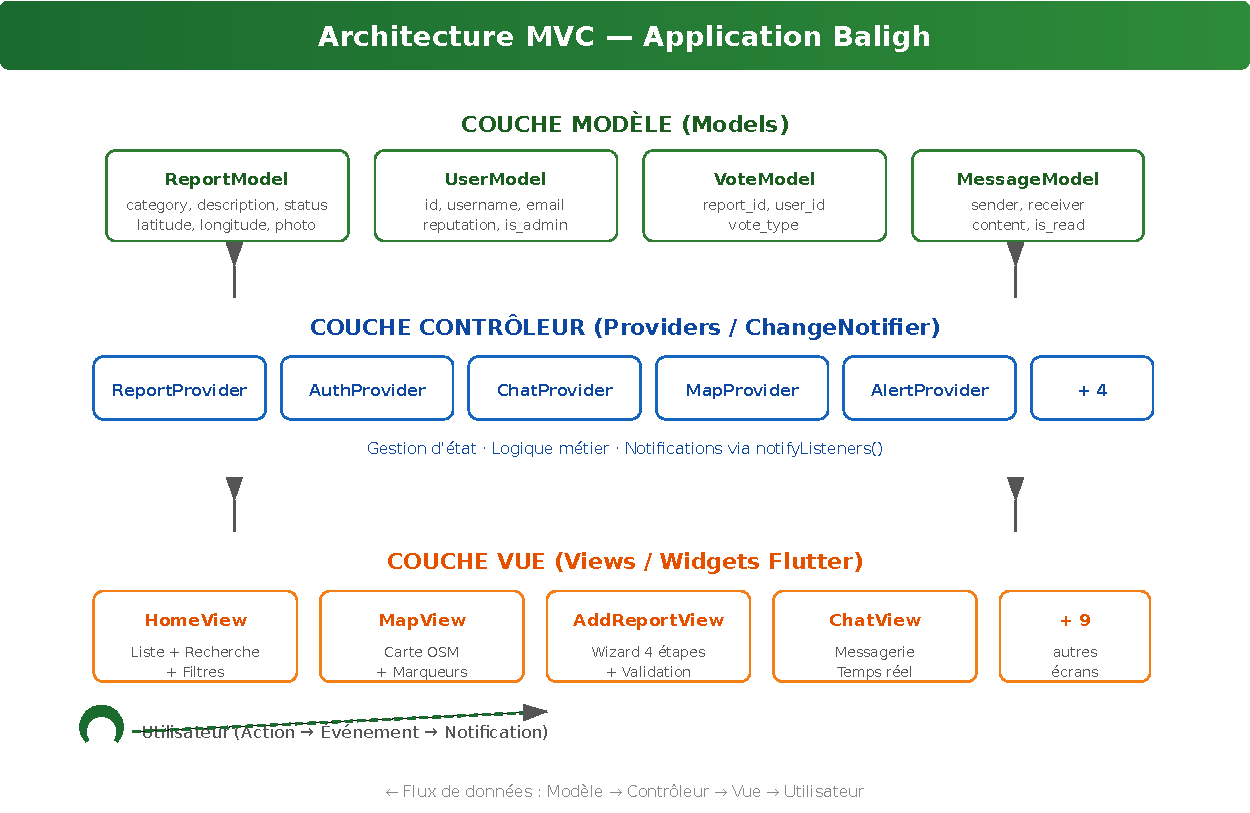
\includegraphics[width=0.85\textwidth]{diagrammes/architecture-mvc.pdf}
    \caption{Architecture MVC de l'application Baligh}
    \label{fig:mvc-diagram}
\end{figure}

Les trois couches principales sont :

\begin{enumerate}
    \item \textbf{Modèles (Models)} : classes Dart avec sérialisation \texttt{toMap()/fromMap()} pour les données : \texttt{ReportModel}, \texttt{UserModel}, \texttt{VoteModel}, \texttt{NotificationModel}, \texttt{MessageModel}.
    
    \item \textbf{Vues (Views)} : widgets Flutter (StatelessWidget/StatefulWidget) qui consomment les providers via \texttt{context.watch}, \texttt{Selector} ou \texttt{Consumer}. 13 écrans principaux.
    
    \item \textbf{Contrôleurs (Controllers)} : classes ChangeNotifier qui détiennent l'état et la logique métier : \texttt{ReportProvider}, \texttt{AuthProvider}, \texttt{ChatProvider}, \texttt{AlertProvider}, \texttt{NavigationProvider}, \texttt{ThemeProvider}, \texttt{LocaleProvider}, \texttt{MapProvider}, \texttt{AddReportProvider}.
\end{enumerate}

En complément :
\begin{itemize}
    \item \textbf{Services} : interfaces abstraites (ex: \texttt{ReportService}) avec implémentations concrètes (\texttt{ReportServiceDb} pour Supabase) ;
    \item \textbf{DAOs} : objets d'accès aux données encapsulant les requêtes Supabase avec paramètres typés (\texttt{ReportDao}, \texttt{UserDao}, \texttt{VoteDao}, \texttt{NotificationDao}, \texttt{MessageDao}).
\end{itemize}

\subsection{Structure du projet}

L'arborescence du projet est organisée comme suit :

\begin{lstlisting}[style=codeblock, caption=Structure du projet Flutter]
lib/
├── main.dart                    # Point d'entree, providers, theme
├── core/
│   ├── database/                # DAOs Supabase (5 classes)
│   │   ├── user_dao.dart        # CRUD utilisateur
│   │   ├── report_dao.dart      # CRUD signalements
│   │   ├── vote_dao.dart        # CRUD votes
│   │   ├── notification_dao.dart # CRUD notifications
│   │   └── message_dao.dart     # CRUD messages
│   ├── models/                  # Modeles (user, vote, notification, message)
│   └── services/                # Services (auth, report, notification, location)
├── models/
│   └── report_model.dart        # ReportModel + categories
├── services/
│   └── report_service.dart      # Interface abstraite
├── controllers/                 # 9 ChangeNotifier providers
├── views/                       # 13 ecrans (dont splash, home, map, ...)
├── widgets/                     # Widgets partages
└── l10n/                        # 3 langues (ARB + Dart generes)
\end{lstlisting}

\section{Stratégie de tests}

La qualité du code a été assurée par plusieurs niveaux de vérification :

\subsection{Tests unitaires}

Les tests unitaires couvrent les modèles et les services :

\begin{itemize}
    \item \textbf{Modèles} : validation de la sérialisation \texttt{toMap()/fromMap()} pour chaque modèle ;
    \item \textbf{Services} : tests des méthodes DAO avec des données mockées ;
    \item \textbf{Contrôleurs} : tests des méthodes CRUD et des transitions d'état.
\end{itemize}

\subsection{Tests d'intégration}

L'intégration avec Supabase a été testée via :
\begin{itemize}
    \item Connexion et authentification (email + Google OAuth) ;
    \item CRUD des signalements (création, lecture, modification, suppression) ;
    \item Système de vote avec double soumission (contrainte UNIQUE) ;
    \item Messagerie temps réel via Supabase Realtime ;
    \item Upload de photos vers Supabase Storage.
\end{itemize}

\subsection{Vérification de la qualité du code}

Plusieurs outils ont été utilisés pour garantir la qualité :

\begin{lstlisting}[style=codeblock, caption=Commandes de verification de qualite]
# Analyse statique du code
flutter analyze

# Formatage du code
dart format lib/

# Verification des types
flutter build apk --release
\end{lstlisting}

\section{Technologies utilisées}
\label{sec:technologies}

\begin{figure}[H]
    \centering
    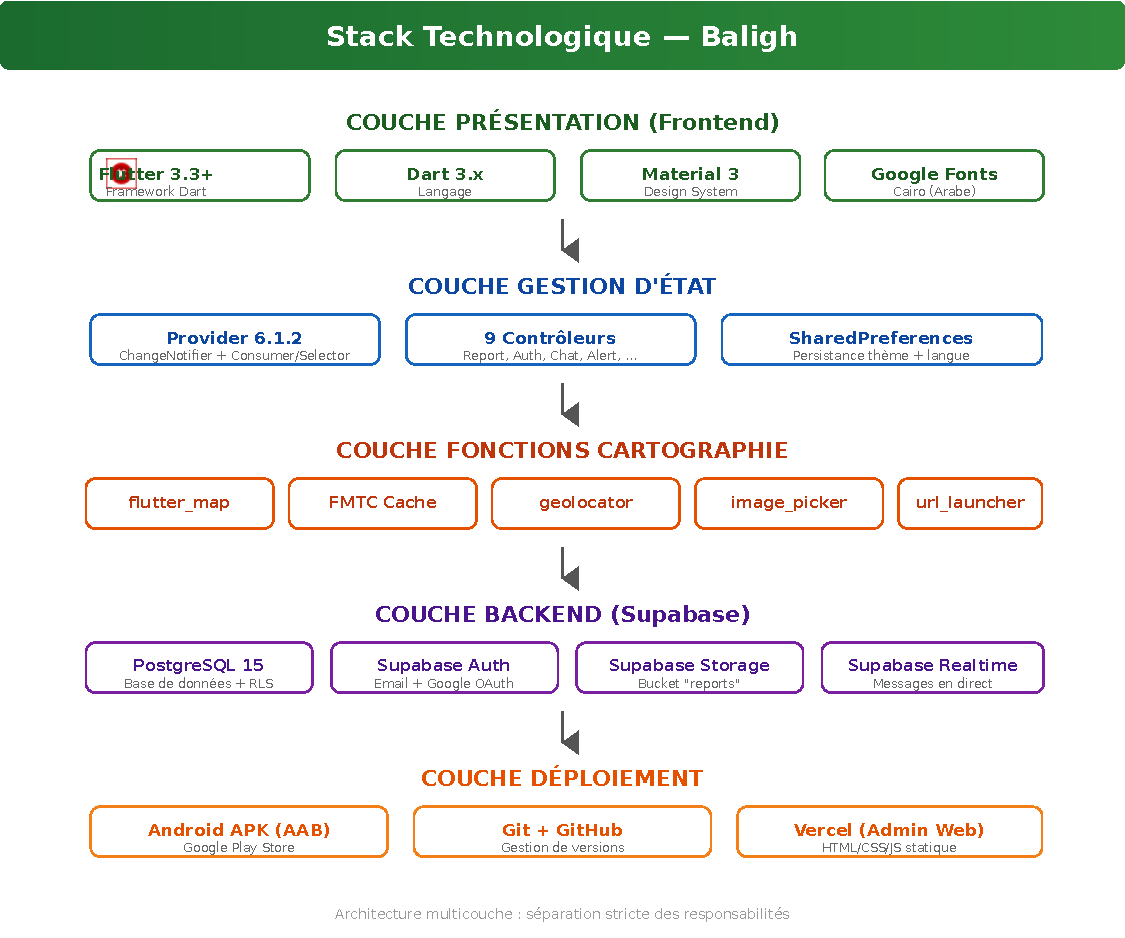
\includegraphics[width=0.85\textwidth]{diagrammes/stack-technologique.pdf}
    \caption{Stack technologique complet de l'application Baligh}
    \label{fig:tech-stack}
\end{figure}

\subsection{Flutter et Dart}

\textbf{Flutter} est un framework de développement d'applications multiplateformes créé par Google. Il permet de développer une application unique pour Android, iOS, Web et desktop à partir d'une même codebase en langage \textbf{Dart}.

Avantages de Flutter pour ce projet :
\begin{itemize}
    \item \textbf{Cross-platform} : une seule application pour Android et iOS ;
    \item \textbf{Hot reload} : développement rapide avec mise à jour instantanée ;
    \item \textbf{Widgets Material 3} : interface moderne et personnalisable ;
    \item \textbf{Grande communauté} : nombreux packages et ressources ;
    \item \textbf{Performance} : compilation native (ARM) pour les mobiles.
\end{itemize}

\subsection{Provider (Gestion d'état)}

\textbf{Provider} est la solution de gestion d'état choisie, conformément au cahier des charges. Il utilise le pattern \textbf{ChangeNotifier} pour notifier les vues des changements d'état.

\begin{lstlisting}[style=codeblock, caption=Exemple de Provider (ReportProvider)]
class ReportProvider extends ChangeNotifier {
  List<ReportModel> _allReports = [];
  ReportCategory? _categoryFilter;
  String _searchQuery = '';
  bool _isLoading = false;

  List<ReportModel> get filteredReports {
    var reports = _allReports;
    if (_categoryFilter != null) {
      reports = reports.where((r) => r.category == _categoryFilter).toList();
    }
    if (_searchQuery.isNotEmpty) {
      reports = reports.where((r) =>
        r.description.toLowerCase().contains(_searchQuery.toLowerCase())
      ).toList();
    }
    return reports;
  }

  Future<void> fetchReports() async {
    _isLoading = true;
    notifyListeners();
    // ... requete Supabase
    _isLoading = false;
    notifyListeners();
  }
}
\end{lstlisting}

\subsection{Supabase (Backend)}

\textbf{Supabase} est une plateforme backend open source qui fournit :
\begin{itemize}
    \item Une base de données \textbf{PostgreSQL} avec API REST ;
    \item L'\textbf{authentification} (email, Google OAuth) ;
    \item Le \textbf{stockage} de fichiers (photos des signalements) ;
    \item La mise à jour en \textbf{temps réel} (Realtime subscriptions) ;
    \item La \textbf{sécurité} via Row Level Security (RLS).
\end{itemize}

Schéma de la base de données :

\begin{figure}[H]
    \centering
    \begin{minipage}{0.9\textwidth}
    \begin{lstlisting}[style=codeblock, caption=Tables de la base Supabase]
-- Utilisateurs
users: id (uuid), username, email, created_at,
       reputation_score, reports_count,
       confirmed_count, is_admin

-- Signalements
reports: id (bigint), user_id (FK), category, description,
         latitude, longitude, address, photo_url,
         created_at, status, confirm_count, deny_count

-- Votes
votes: id (bigint), report_id (FK), user_id (FK),
       vote_type, created_at
       UNIQUE(report_id, user_id)

-- Notifications
notifications: id (bigint), user_id (FK), report_id (FK),
               message, is_read, created_at

-- Messages
messages: id (bigint), report_id (FK), sender_id (FK),
          receiver_id (FK), content, is_read, created_at
\end{lstlisting}
    \end{minipage}
    \caption{Structure de la base de données PostgreSQL}
    \label{fig:schema-bd}
\end{figure}

\subsection{OpenStreetMap et flutter\_map}

Pour la cartographie, nous utilisons \textbf{OpenStreetMap} (OSM) via le package \texttt{flutter\_map}, avec \texttt{flutter\_map\_tile\_caching} (FMTC) pour la mise en cache des tuiles :

\begin{itemize}
    \item Stratégie : \texttt{cacheFirst} -- tuiles servies depuis le cache si disponibles ;
    \item Durée de validité : 30 jours ;
    \item Zoom maximal : 19 ;
    \item Aucune clé API requise (contrairement à Google Maps).
\end{itemize}

\subsection{Internationalisation (i18n)}

L'internationalisation est gérée avec \texttt{flutter\_localizations} et \texttt{intl} via des fichiers ARB :

\begin{itemize}
    \item \texttt{app\_ar.arb} -- Arabe (RTL) ;
    \item \texttt{app\_fr.arb} -- Français (LTR) ;
    \item \texttt{app\_en.arb} -- Anglais (LTR).
\end{itemize}

Plus de 95 clés de traduction sont réparties en 12 catégories (navigation, accueil, signalement, catégories, etc.). Le choix de langue est persisté via \texttt{SharedPreferences}.

\section{Diagramme de navigation}

L'application utilise une navigation à deux niveaux :

\begin{enumerate}
    \item \textbf{Shell persistant} : \texttt{MainLayout} avec \texttt{IndexedStack} (4 onglets) + \texttt{BottomAppBar} + FAB central. La commutation d'onglets se fait via \texttt{NavigationProvider} (enum \texttt{AppTab}).
    \item \textbf{Routes push} : navigation standard avec \texttt{Navigator.push()} pour les écrans secondaires : \texttt{AddReportView} (depuis FAB), \texttt{ReportDetailView} (depuis cartes de signalement), \texttt{EmergencyNumbersView} (depuis SOS FAB / Compte), \texttt{ChatView} et \texttt{ConversationsView} (depuis icône chat).
\end{enumerate}

\begin{figure}[H]
    \centering
    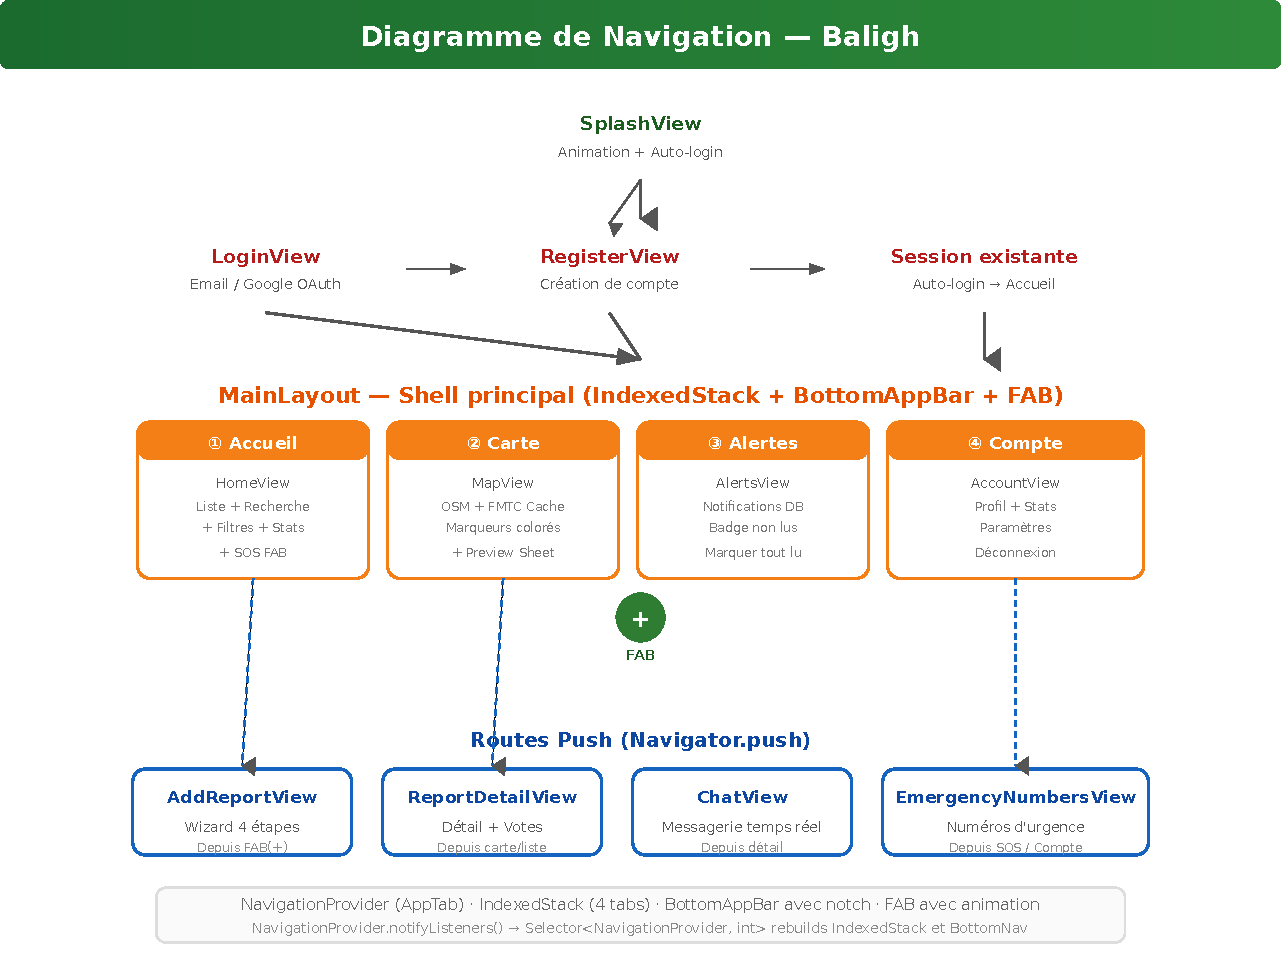
\includegraphics[width=0.9\textwidth]{diagrammes/navigation-app.pdf}
    \caption{Diagramme de navigation de l'application Baligh}
    \label{fig:navigation}
\end{figure}

Les 4 onglets du shell principal sont :
\begin{enumerate}
    \item \textbf{Accueil} (\texttt{HomeView}) -- flux principal des signalements, barre de recherche, filtres, statistiques ;
    \item \textbf{Carte} (\texttt{MapView}) -- carte interactive OpenStreetMap avec marqueurs ;
    \item \textbf{Alerte} (\texttt{AlertsView}) -- notifications et alertes ;
    \item \textbf{Compte} (\texttt{AccountView}) -- profil, paramètres, numéros d'urgence.
\end{enumerate}

\section{Base de données et migrations}

La base de données Supabase contient 5 tables principales. La migration est gérée via le fichier \texttt{supabase\_migration.sql} qui définit :

\begin{itemize}
    \item Les tables avec leurs contraintes (clés primaires, clés étrangères, contraintes UNIQUE) ;
    \item Les index pour optimiser les requêtes ;
    \item Les politiques RLS (Row Level Security) pour chaque table ;
    \item Les fonctions RPC \texttt{SECURITY DEFINER} pour les opérations nécessitant un contournement de RLS ;
    \item Le bucket de stockage \texttt{reports} avec ses politiques d'accès.
\end{itemize}

\subsection{Diagramme entité-relation}

\begin{lstlisting}[style=codeblock, caption=Schéma relationnel de la base de donnees]
users (id, username, email, created_at, reputation_score,
       reports_count, confirmed_count, is_admin)
    |--< reports (user_id FK)
    |--< votes (user_id FK)
    |--< notifications (user_id FK)
    |--< messages (sender_id FK, receiver_id FK)

reports (id, user_id FK, category, description, latitude,
         longitude, address, photo_url, created_at, status,
         confirm_count, deny_count)
    |--< votes (report_id FK)
    |--< notifications (report_id FK)
    |--< messages (report_id FK)

votes (id, report_id FK, user_id FK, vote_type, created_at)
    UNIQUE(report_id, user_id) -- 1 vote/user/report

notifications (id, user_id FK, report_id FK, message, is_read, created_at)

messages (id, report_id FK, sender_id FK, receiver_id FK,
          content, is_read, created_at)
\end{lstlisting}

\subsection{Politiques RLS}

Les politiques Row Level Security constituent un élément central de la sécurité de l'application :

{\small
\begin{longtable}{|p{2.5cm}|p{2.5cm}|p{9.5cm}|}
    \caption{Politiques RLS de la base de données}
    \label{tab:rls}\\
    \hline
    \rowcolor{supnumgreen!20}
    \textbf{Table} & \textbf{Opération} & \textbf{Politique} \\
    \hline
    \endhead
    \hline
    \endfoot
    reports & SELECT & Tout utilisateur authentifié \\
    \hline
    reports & INSERT & Créateur = utilisateur connecté \\
    \hline
    reports & UPDATE & Créateur ou administrateur \\
    \hline
    reports & DELETE & Créateur ou administrateur \\
    \hline
    votes & SELECT & Tout utilisateur authentifié \\
    \hline
    votes & INSERT & auth.uid() = user\_id \\
    \hline
    votes & UPDATE & auth.uid() = user\_id \\
    \hline
    notifications & SELECT & auth.uid() = user\_id \\
    \hline
    notifications & INSERT & Fonction SECURITY DEFINER \\
    \hline
    messages & SELECT & Participant à la conversation \\
    \hline
    messages & INSERT & Utilisateur authentifié \\
    \hline
    messages & UPDATE & Destinataire \\
    \hline
\end{longtable}
}

\section{Sécurité}

La sécurité est assurée à plusieurs niveaux :

\begin{itemize}
    \item \textbf{Row Level Security (RLS)} : chaque utilisateur ne voit/modifie que ses propres données ;
    \item \textbf{SECURITY DEFINER} : fonctions RPC contournant RLS pour les mises à jour de compteurs de votes et la création de notifications ;
    \item \textbf{Authentification Supabase} : gestion des tokens JWT, sessions persistantes ;
    \item \textbf{Google OAuth} : authentification sécurisée via Google Sign-In ;
    \item \textbf{Stockage sécurisé} : bucket \texttt{reports} avec politiques RLS (upload/lecture/suppression).
\end{itemize}

% =====================================================
% CHAPITRE 5 : FONCTIONNALITÉS DÉVELOPPÉES
% =====================================================
\chapter{Fonctionnalités développées}

\section{Authentification et gestion des utilisateurs}

\subsection{Écran de bienvenue}

\begin{figure}[!ht]
    \centering
    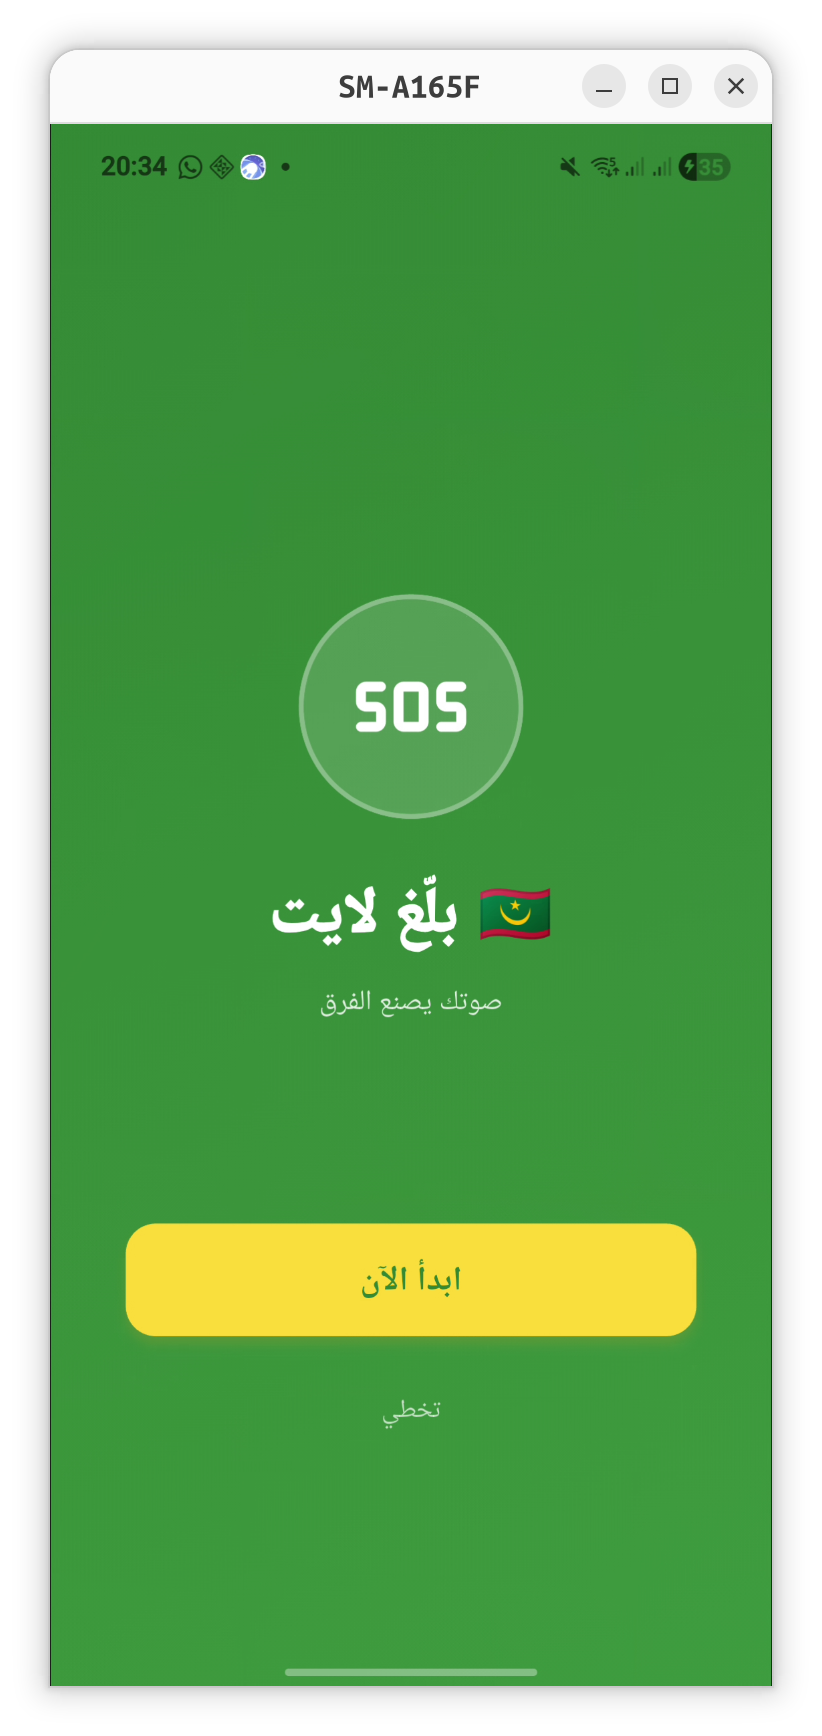
\includegraphics[width=0.35\textwidth]{captures-application/splash.png}
    \caption{Écran de bienvenue -- démarrage et auto-login}
    \label{fig:welcome}
\end{figure}

\noindent Si une session active existe, l'utilisateur est automatiquement redirigé vers l'accueil sans passer par cet écran.

\subsection{Écran de connexion}

L'écran de connexion permet aux utilisateurs de s'authentifier via :
\begin{itemize}
    \item Email et mot de passe (Supabase Auth) ;
    \item Google Sign-In (OAuth 2.0).
\end{itemize}

L'auto-login est géré automatiquement : si une session active existe, l'utilisateur est redirigé directement vers l'accueil.

\begin{figure}[H]
    \centering
    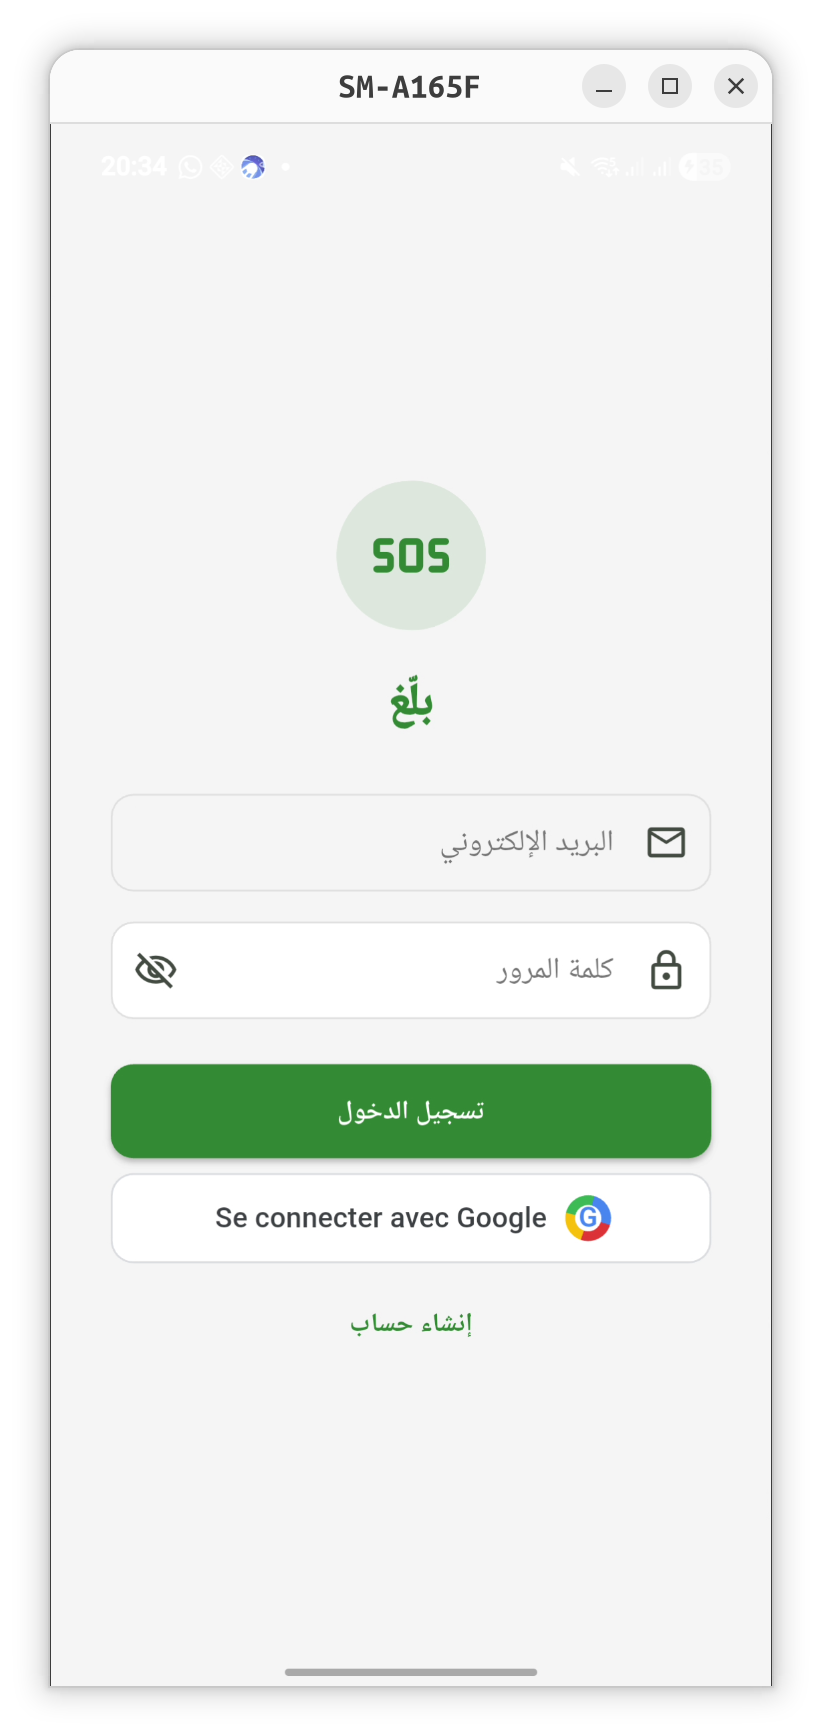
\includegraphics[width=0.4\textwidth]{captures-application/connexion.png}
    \caption{Écran de connexion}
    \label{fig:connexion}
\end{figure}

\subsection{Écran d'inscription}

L'écran d'inscription permet la création d'un compte avec email, mot de passe et nom d'utilisateur.

\begin{figure}[H]
    \centering
    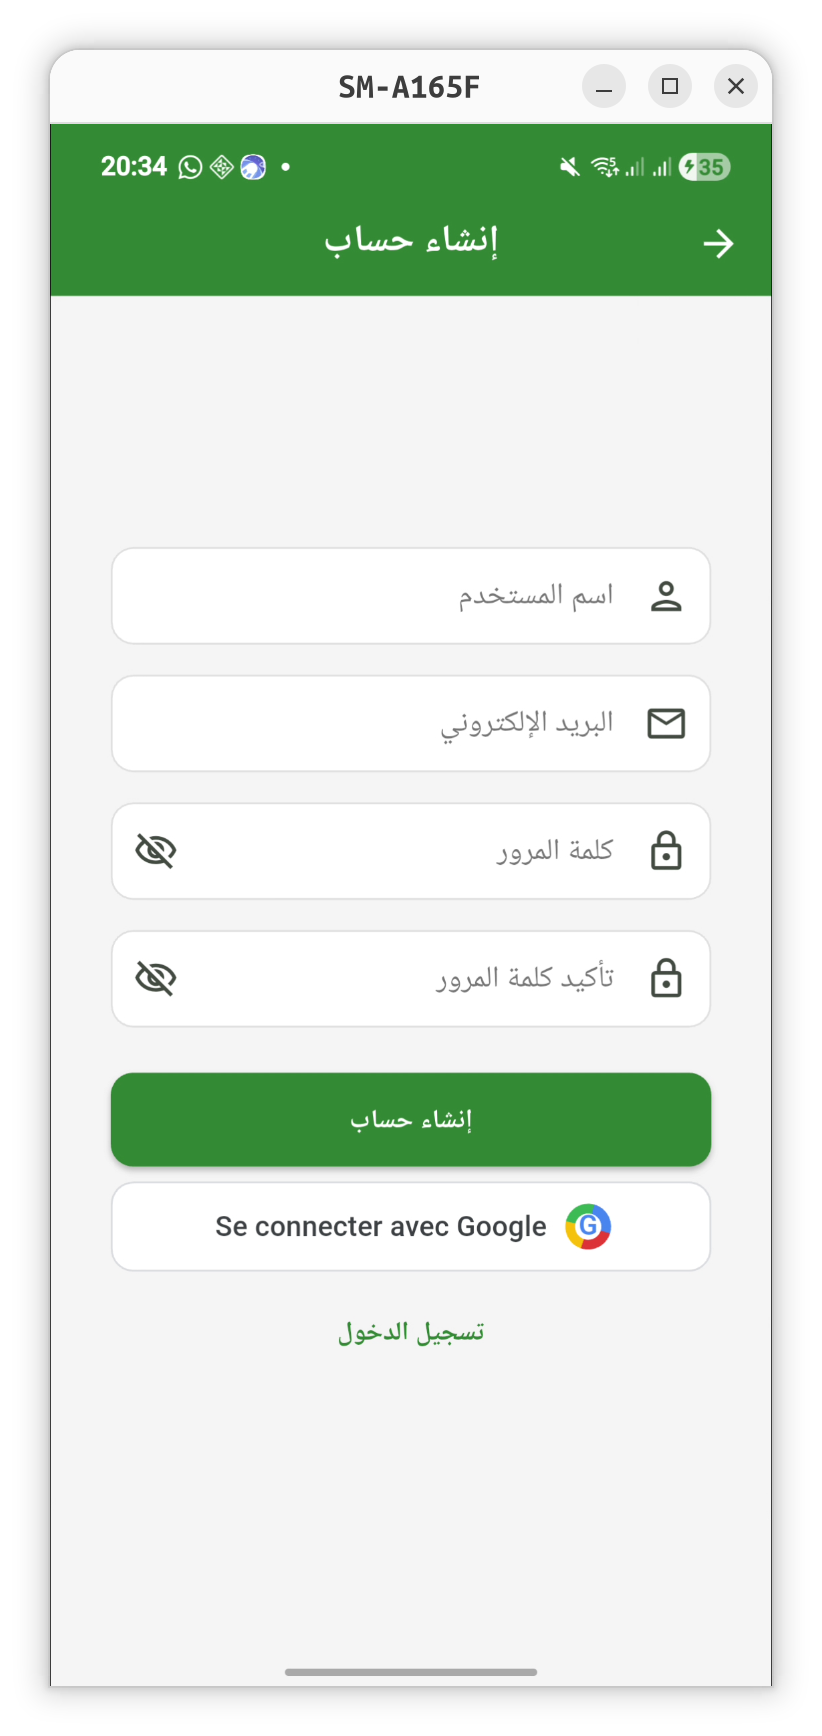
\includegraphics[width=0.4\textwidth]{captures-application/register.png}
    \caption{Écran d'inscription}
    \label{fig:register}
\end{figure}

\section{Accueil et flux de signalements}

\subsection{Page d'accueil}

La page d'accueil présente :
\begin{itemize}
    \item Une \textbf{SliverAppBar} avec gradient, titre et icône de notifications ;
    \item Une \textbf{barre de statistiques} (total, en attente, validés) ;
    \item Des \textbf{filtres par catégorie} (12 catégories) ;
    \item Une \textbf{barre de recherche} textuelle ;
    \item La \textbf{liste des signalements} avec animation d'entrée (staggered fade + slide) ;
    \item Un \textbf{bouton SOS} (rouge) pour les numéros d'urgence.
\end{itemize}

\begin{figure}[H]
    \centering
    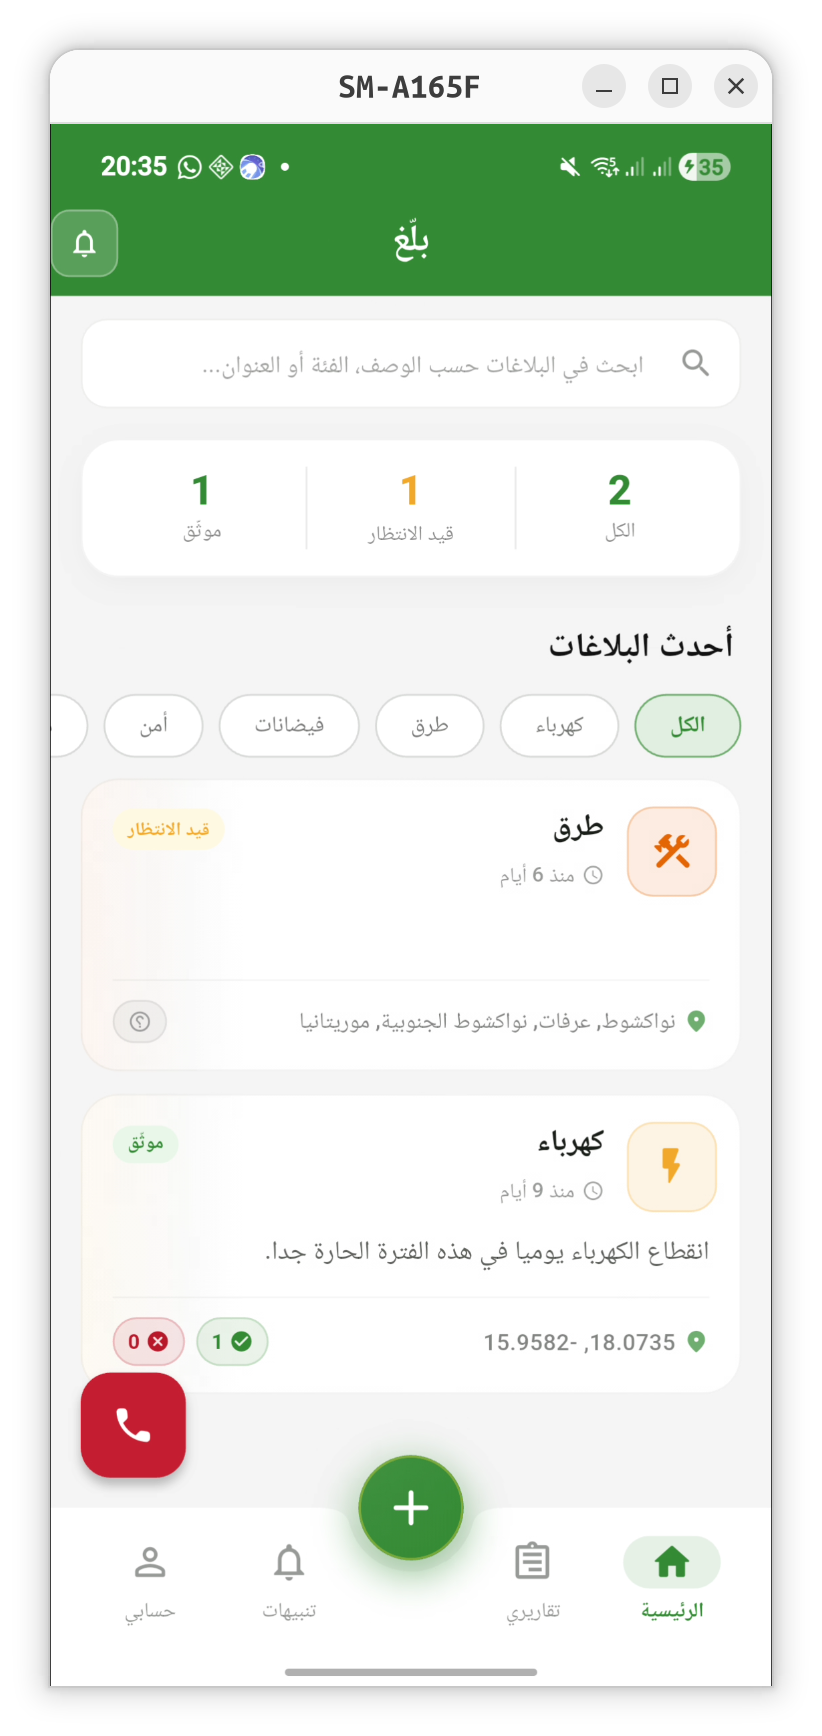
\includegraphics[width=0.4\textwidth]{captures-application/acceuil.png}
    \caption{Page d'accueil avec la liste des signalements}
    \label{fig:acceuil}
\end{figure}

\section{Création d'un signalement (Assistant en 4 étapes)}

L'ajout d'un signalement se fait via un assistant (wizard) en 4 étapes, accessible depuis le bouton FAB central.

\begin{figure}[H]
    \centering
    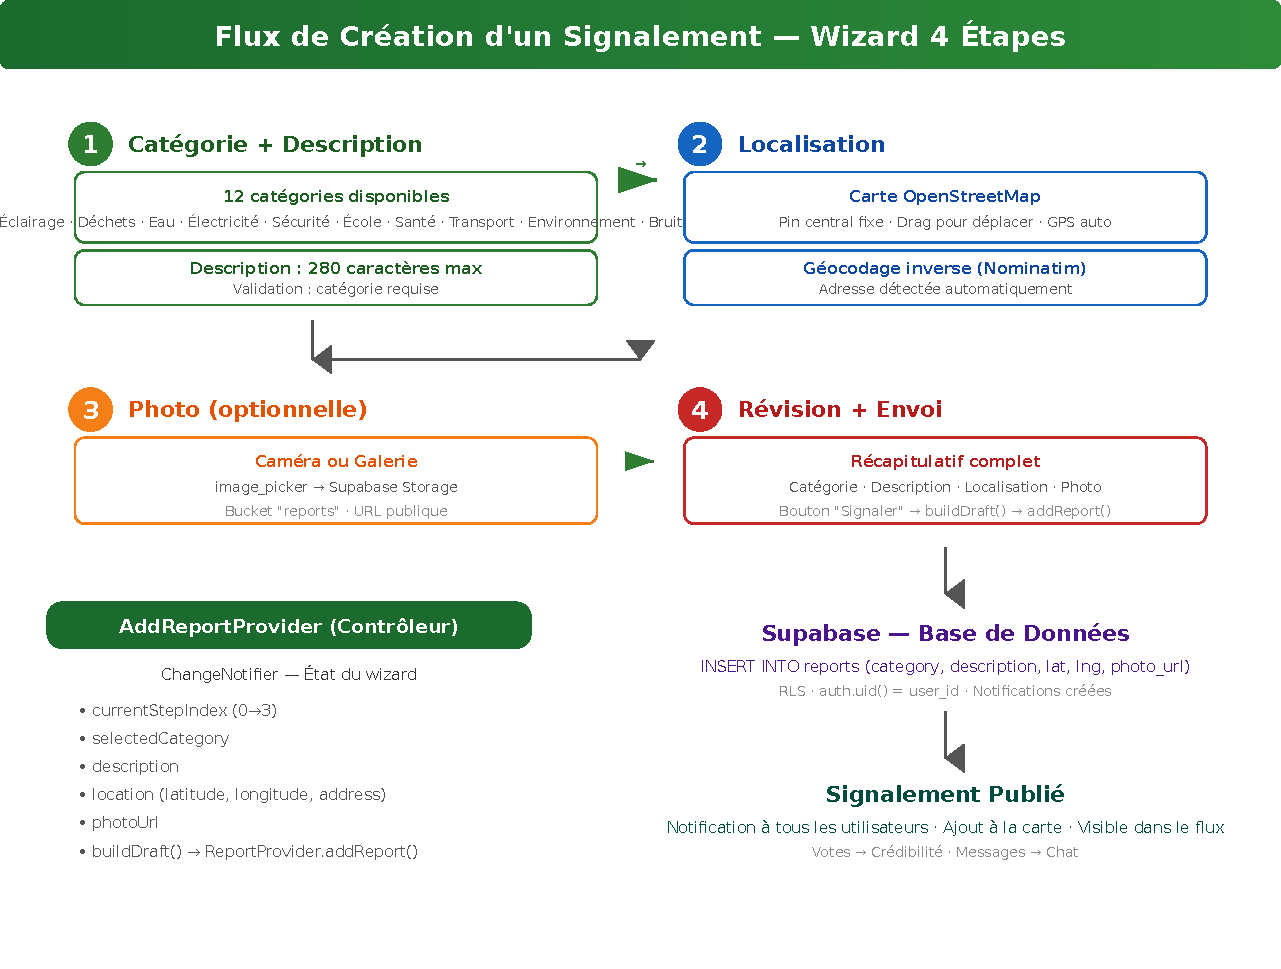
\includegraphics[width=0.92\textwidth]{diagrammes/flow-signalement.pdf}
    \caption{Flux complet de création d'un signalement (Wizard 4 étapes)}
    \label{fig:flow-signalement}
\end{figure}

\subsection{Étape 1 : Catégorie et description}

L'utilisateur sélectionne une catégorie parmi 12 options et rédige une description (280 caractères max).

\begin{figure}[H]
    \centering
    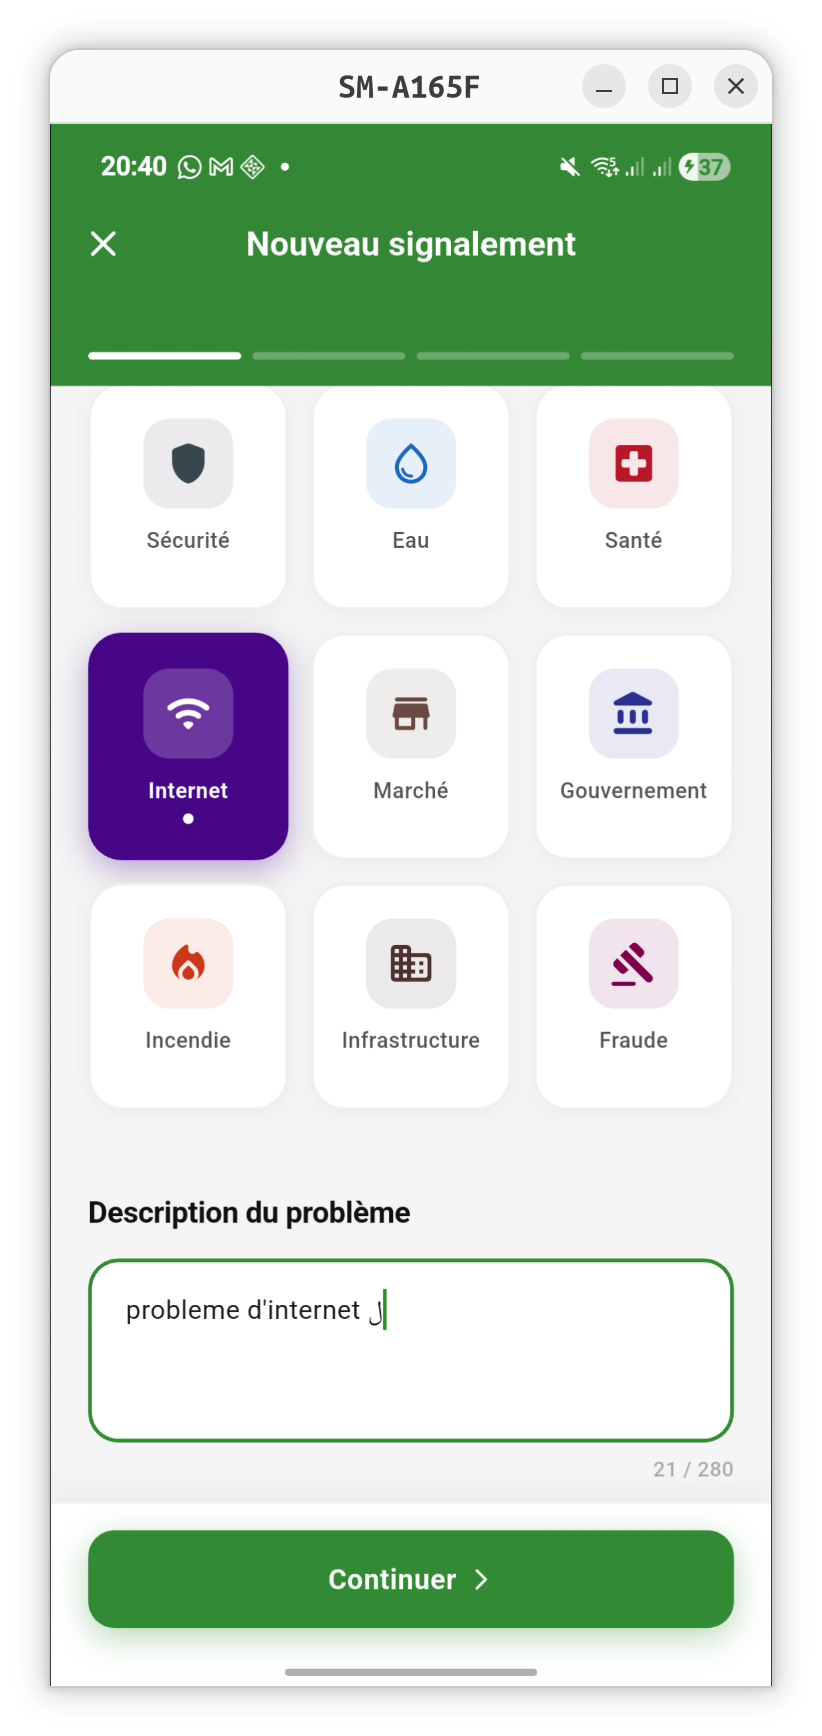
\includegraphics[width=0.4\textwidth]{captures-application/nouveau-signalement.png}
    \caption{Étape 1 : Sélection de la catégorie et description}
    \label{fig:nouveau-signalement}
\end{figure}

\subsection{Étape 2 : Localisation sur la carte}

L'utilisateur positionne le signalement sur une carte OpenStreetMap. La localisation GPS automatique est supportée. Une adresse est générée via le service de géocodage inverse Nominatim.

\begin{figure}[H]
    \centering
    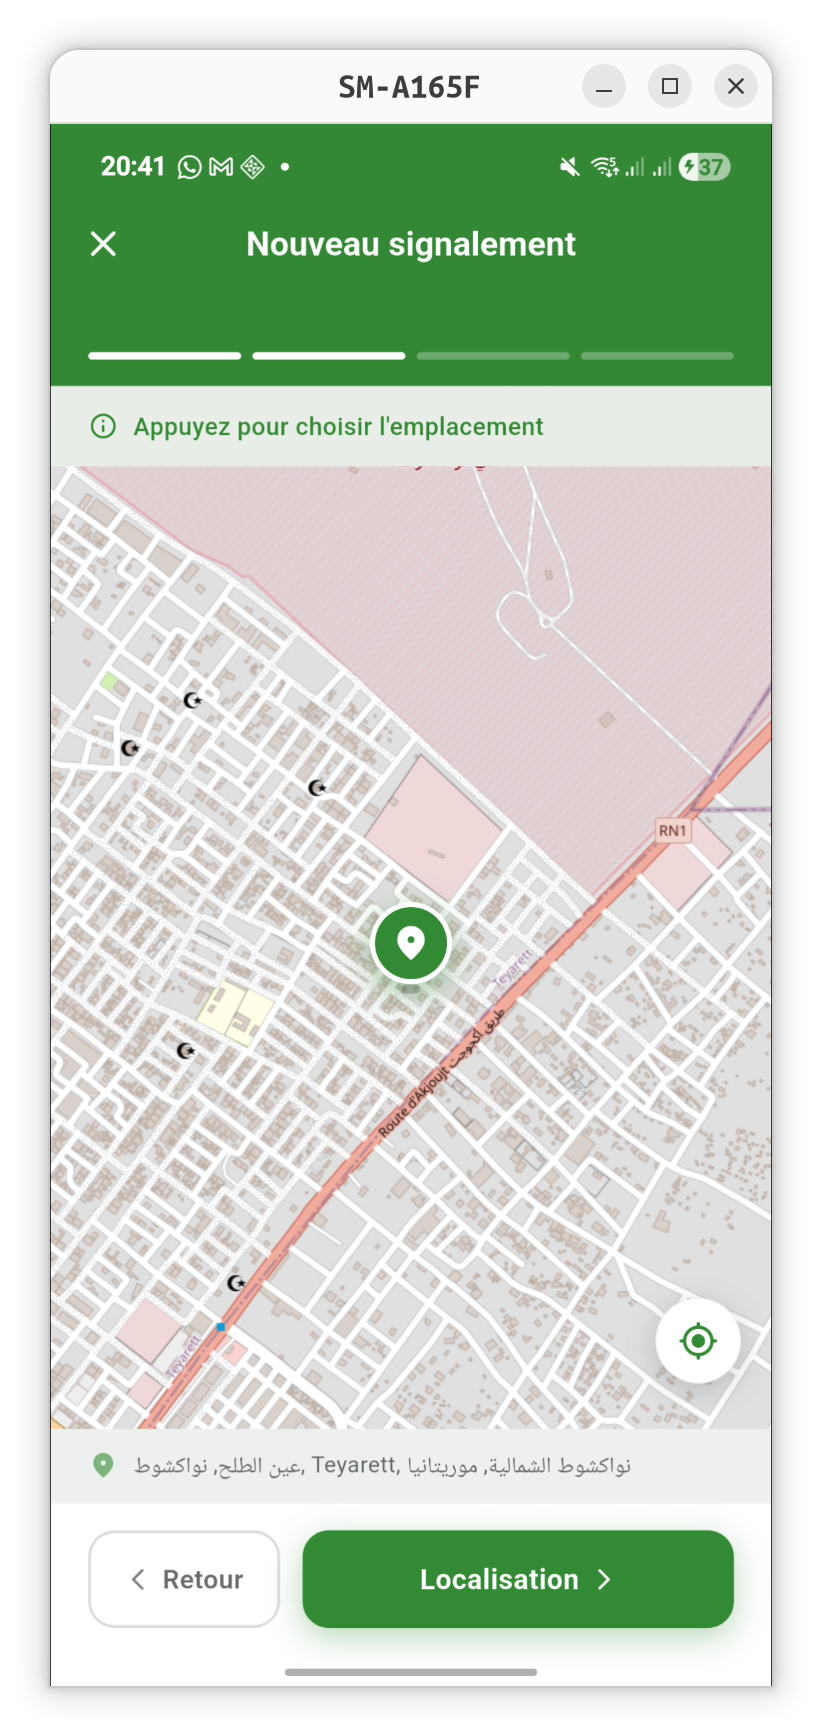
\includegraphics[width=0.4\textwidth]{captures-application/carte-maps.png}
    \caption{Étape 2 : Sélection de la localisation sur la carte}
    \label{fig:carte-maps}
\end{figure}

\subsection{Étape 3 : Photo}

L'utilisateur peut prendre une photo ou choisir une image depuis la galerie. La photo est uploadée vers Supabase Storage (bucket \texttt{reports}) et l'URL publique est sauvegardée dans le signalement.

\begin{figure}[H]
    \centering
    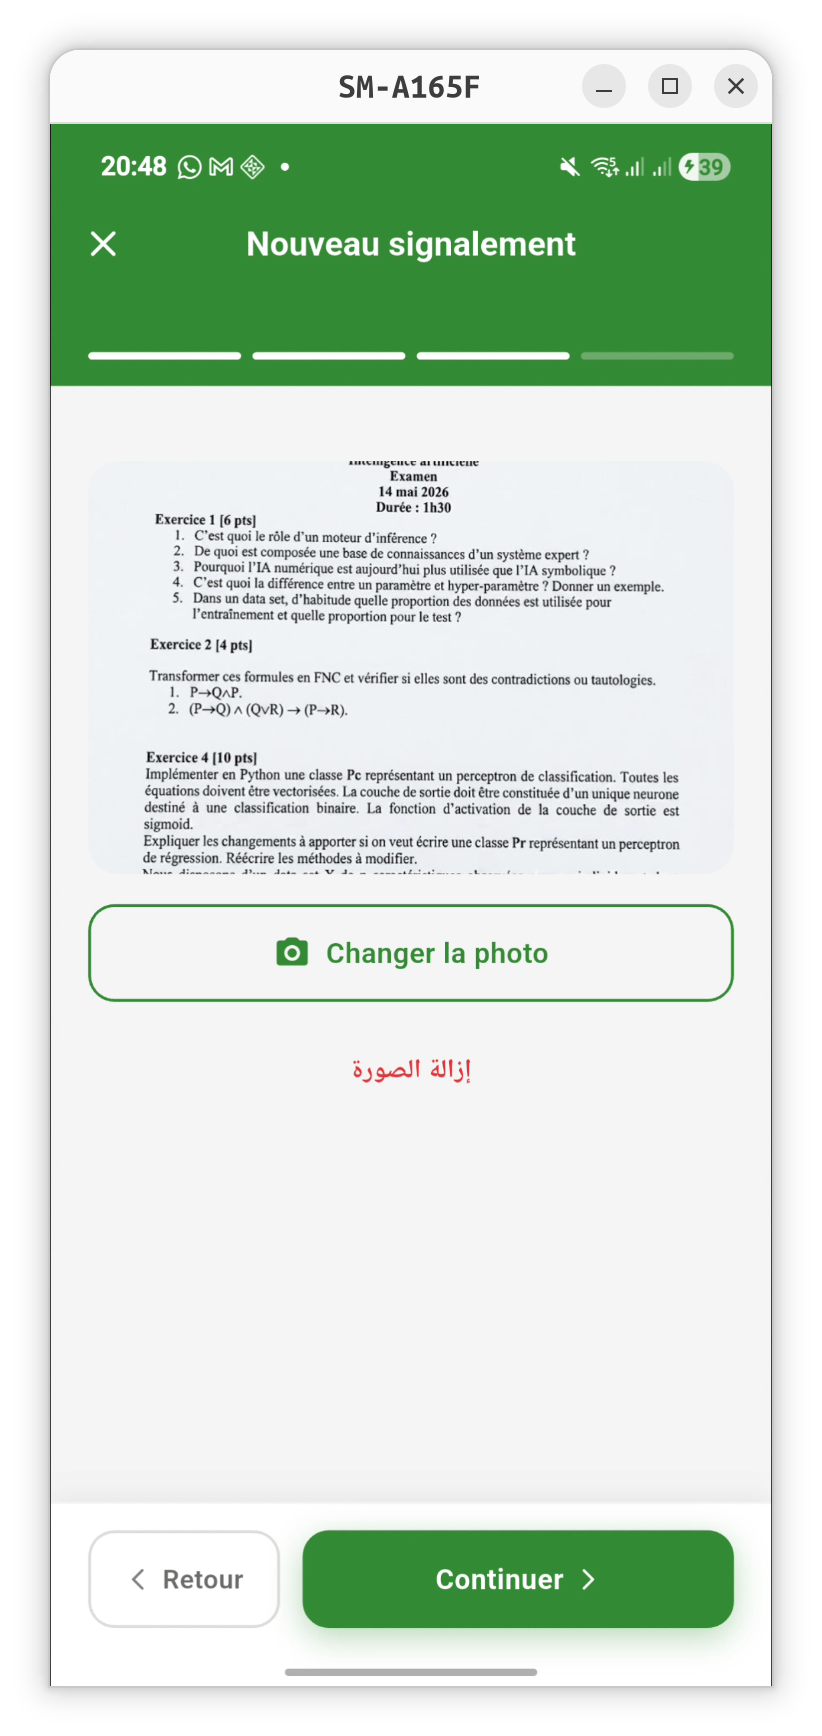
\includegraphics[width=0.4\textwidth]{captures-application/prendre-photo.png}
    \caption{Étape 3 : Prise de photo}
    \label{fig:prendre-photo}
\end{figure}

\subsection{Étape 4 : Révision et envoi}

Avant l'envoi, l'utilisateur peut réviser l'ensemble des informations (catégorie, description, localisation, photo). La soumission déclenche l'enregistrement en base de données via \texttt{ReportProvider.addReport()}.

\begin{figure}[H]
    \centering
    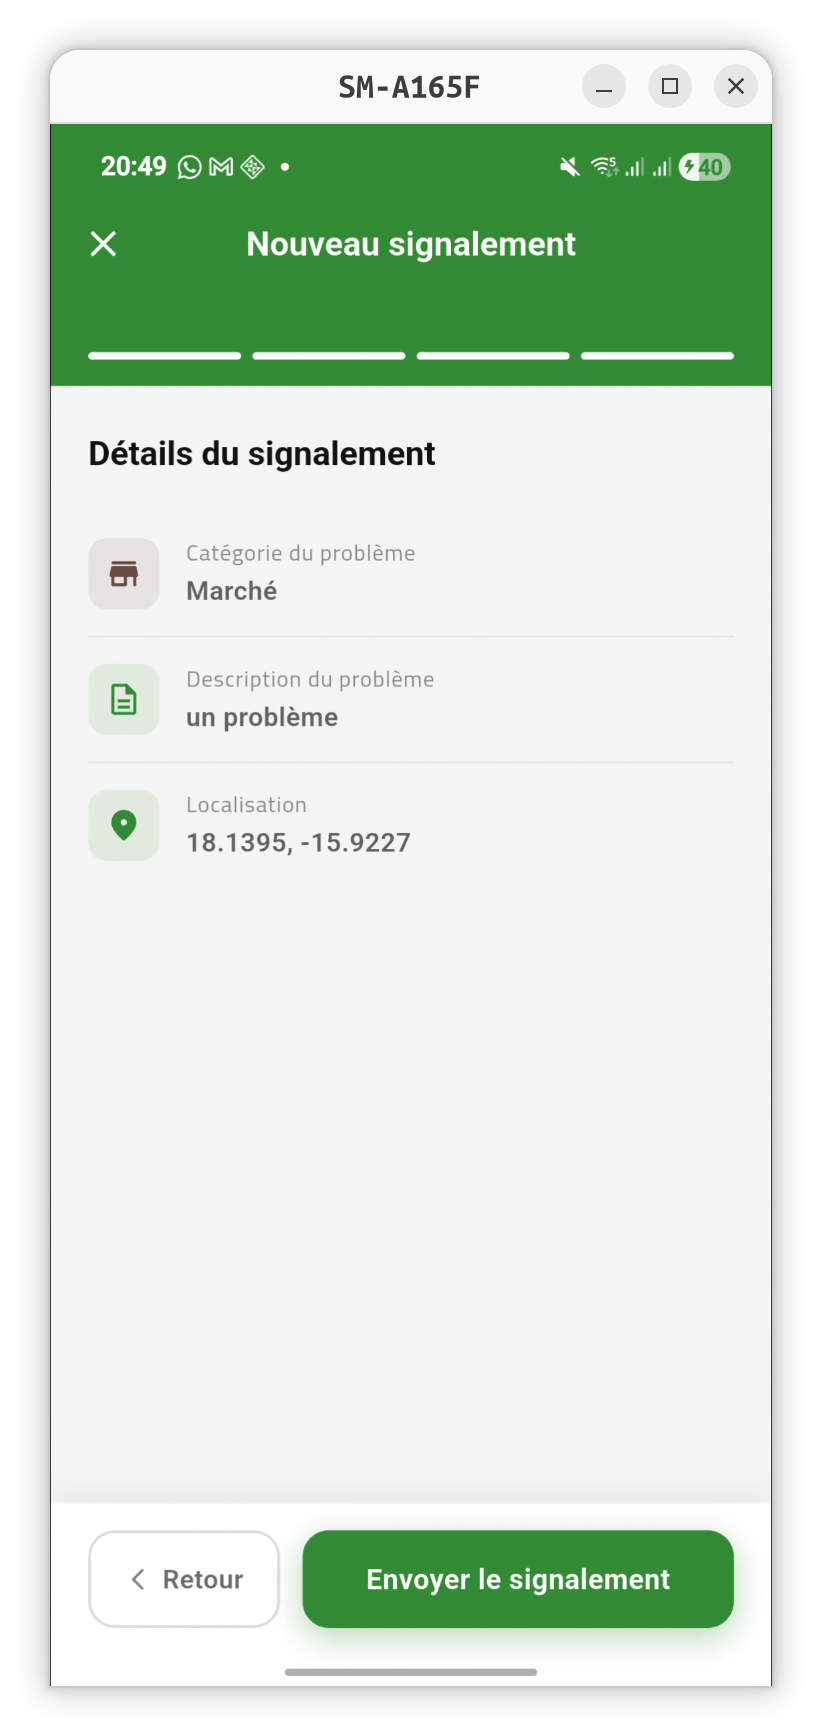
\includegraphics[width=0.4\textwidth]{captures-application/envoie-signalement.png}
    \caption{Étape 4 : Révision et envoi du signalement}
    \label{fig:envoie-signalement}
\end{figure}

\section{Carte interactive}

La carte interactive (deuxième onglet) affiche tous les signalements sous forme de marqueurs colorés par catégorie. Les fonctionnalités incluent :
\begin{itemize}
    \item Tuiles OpenStreetMap avec cache FMTC (30 jours) ;
    \item Marqueurs avec icônes et couleurs par catégorie ;
    \item Barre de recherche avec suggestion ;
    \item Filtres par catégorie ;
    \item Sélection d'un marqueur → aperçu (preview sheet) avec votes ;
    \item Bouton de localisation (recentrage sur la position GPS).
\end{itemize}

\begin{figure}[H]
    \centering
    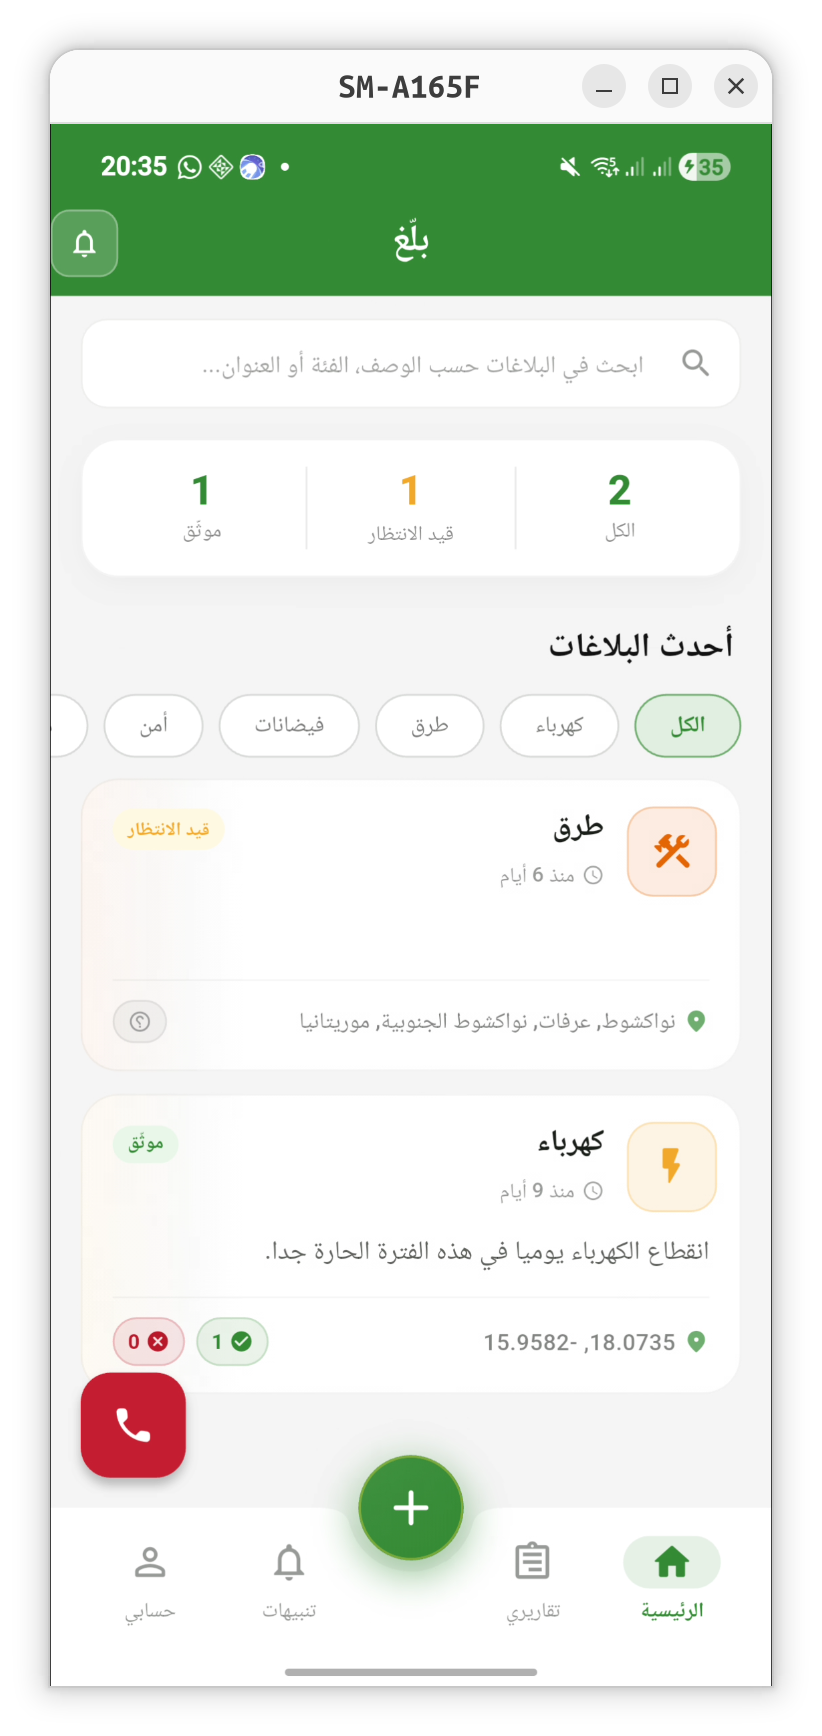
\includegraphics[width=0.4\textwidth]{captures-application/acceuil.png}
    \caption{Vue des signalements sur la carte interactive}
    \label{fig:carte-maps2}
\end{figure}

\section{Détail d'un signalement}

L'écran de détail présente :
\begin{itemize}
    \item En-tête avec icône de catégorie et statut ;
    \item Photo (si disponible) ;
    \item Section informations (catégorie, date, emplacement) ;
    \item Description complète ;
    \item Barre de crédibilité (pourcentage) ;
    \item Boutons Confirmer/Infirmer (vote) ;
    \item Coordonnées avec lien Google Maps ;
    \item Bouton de partage ;
    \item Icône de chat dans l'AppBar (messagerie).
\end{itemize}

\begin{figure}[H]
    \centering
    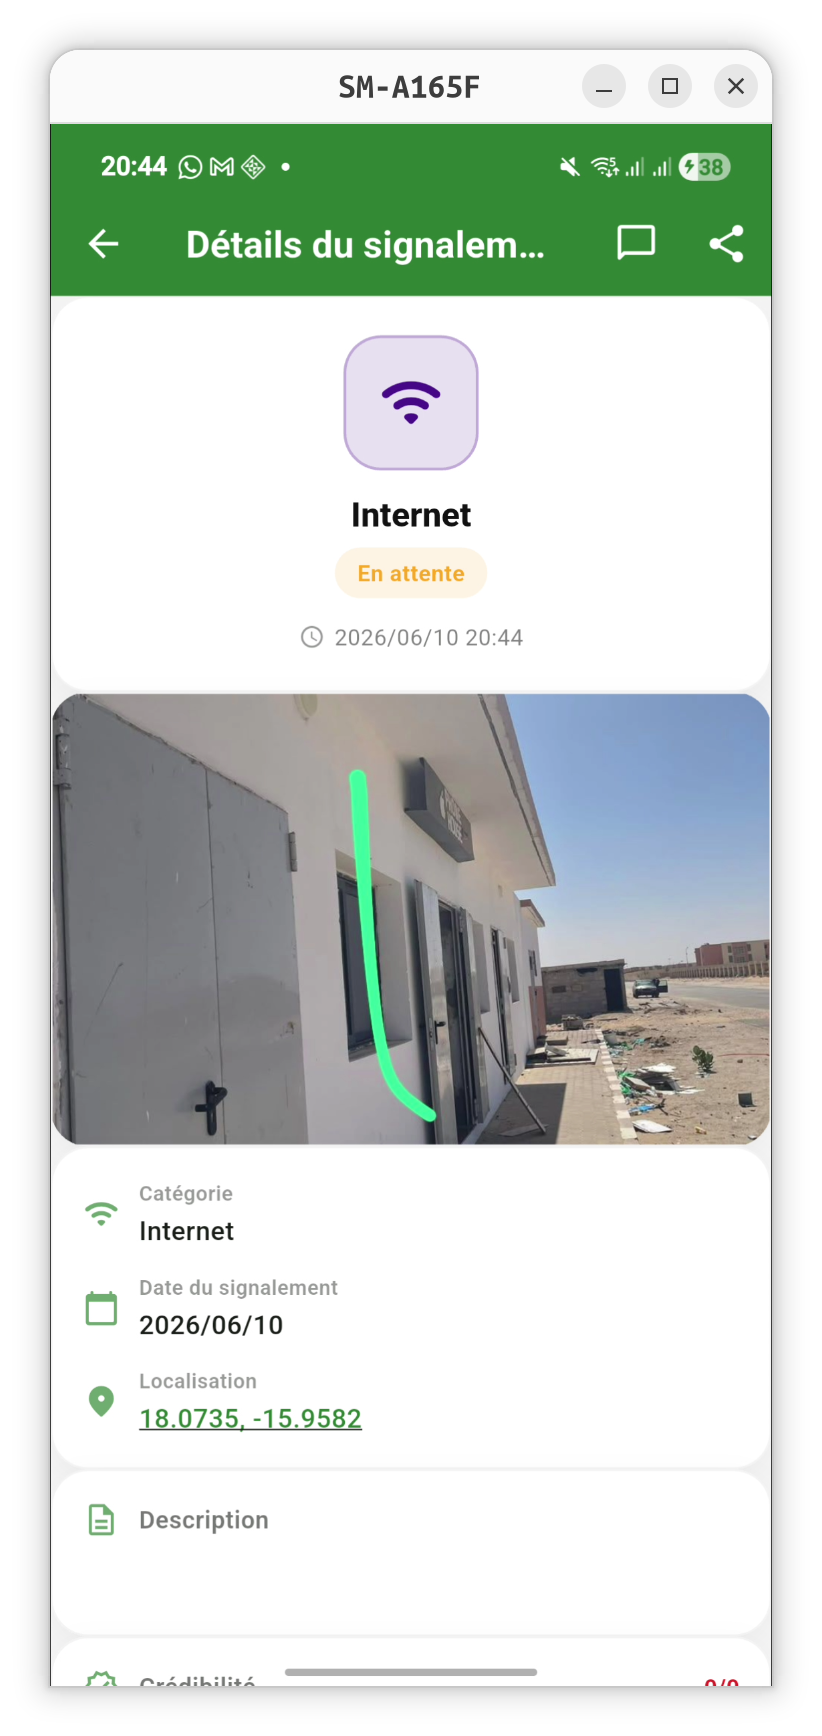
\includegraphics[width=0.4\textwidth]{captures-application/detail_du_signalement.png}
    \caption{Écran de détail d'un signalement}
    \label{fig:detail-signalement}
\end{figure}

\section{Mes signalements}

L'onglet "Mes signalements" affiche la liste des signalements de l'utilisateur connecté, avec :
\begin{itemize}
    \item Filtre par statut (bottom sheet) ;
    \item Boutons d'édition et de suppression (propres signalements) ;
    \item Navigation vers le détail.
\end{itemize}

\begin{figure}[H]
    \centering
    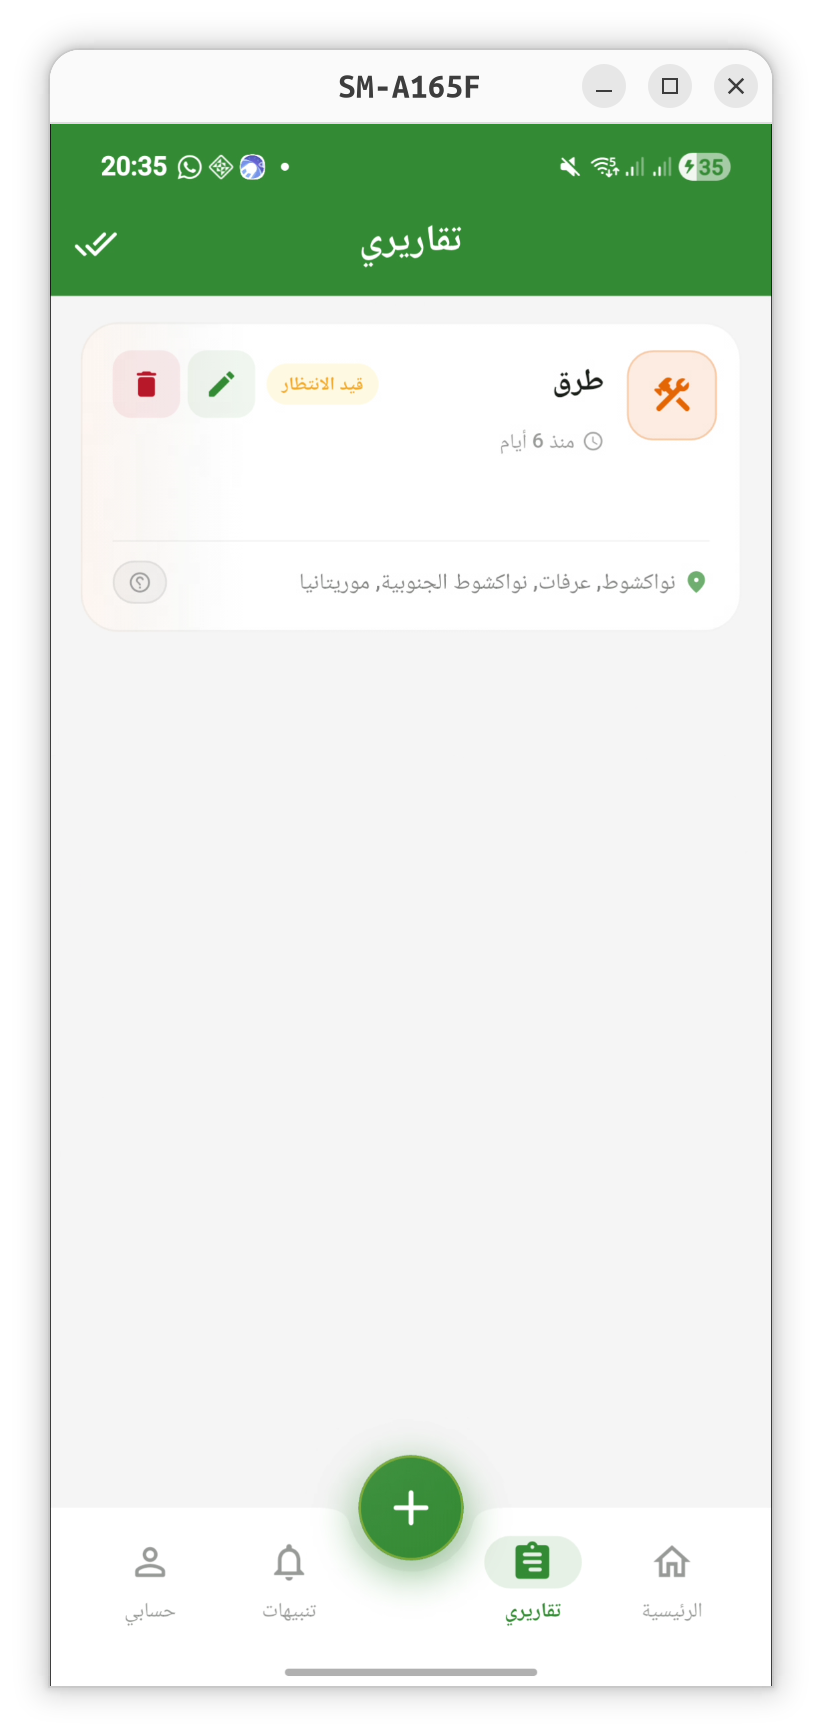
\includegraphics[width=0.4\textwidth]{captures-application/mes-signales.png}
    \caption{Liste de mes signalements}
    \label{fig:mes-signales}
\end{figure}

\section{Notifications (Alertes)}

L'onglet "Alertes" affiche les notifications en provenance de la base de données (table \texttt{notifications}). Une notification est créée pour chaque nouveau signalement (sauf pour l'auteur). Fonctionnalités :
\begin{itemize}
    \item Liste des notifications avec date ;
    \item Indicateur de lecture (non lu/lu) ;
    \item Marquer tout comme lu ;
    \item Pull-to-refresh ;
    \item Badge de compteur non lu.
\end{itemize}

\begin{figure}[H]
    \centering
    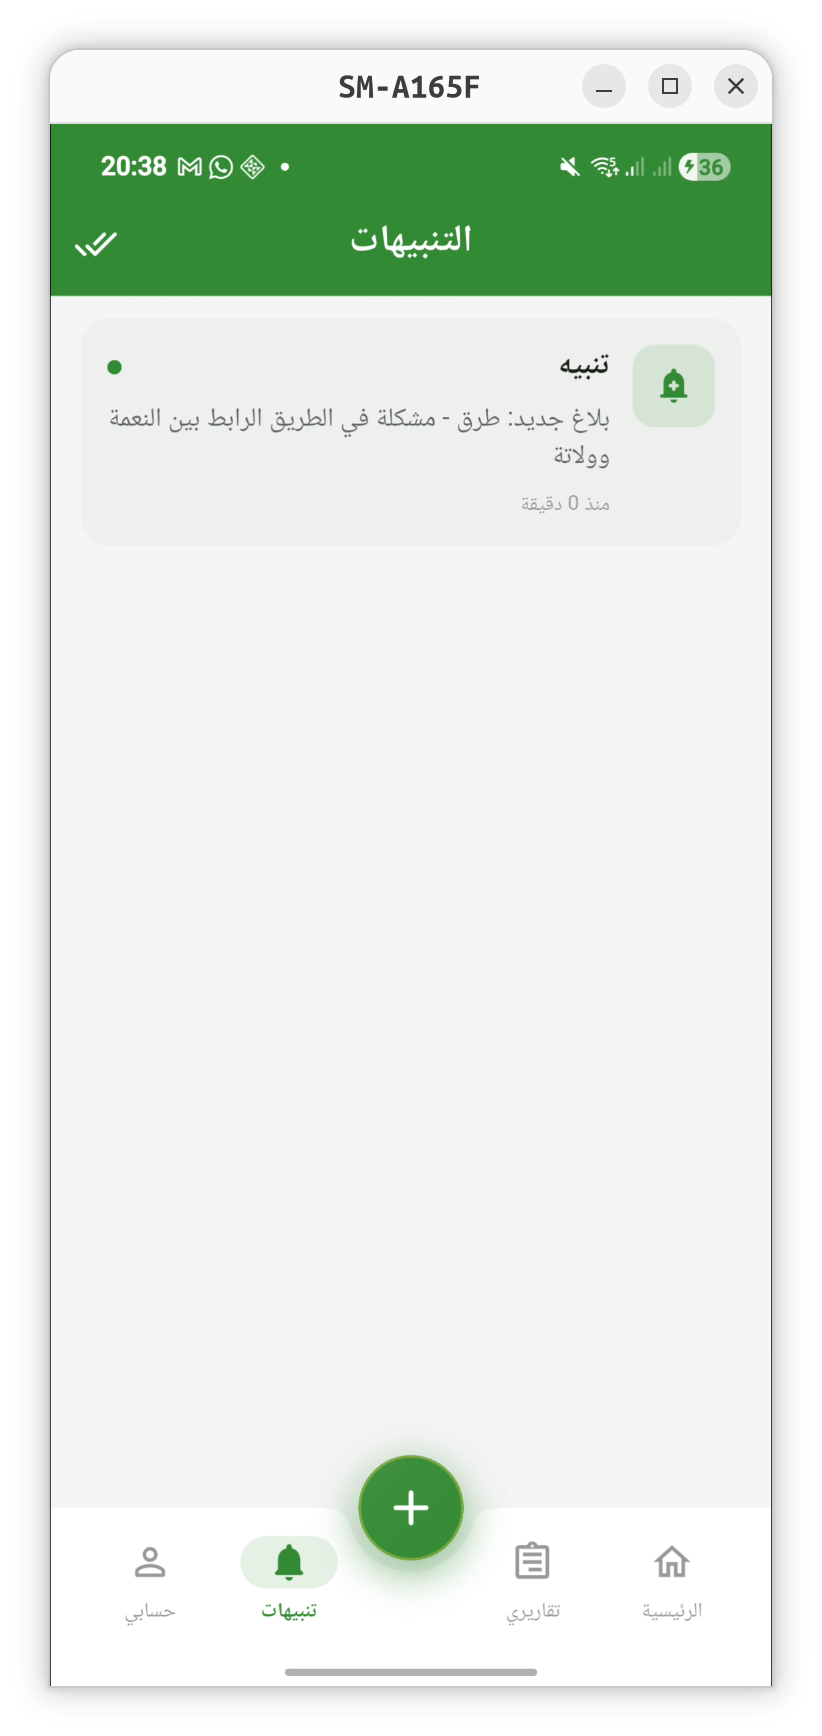
\includegraphics[width=0.4\textwidth]{captures-application/alert.png}
    \caption{Écran des notifications (alertes)}
    \label{fig:alertes}
\end{figure}

\section{Profil et compte}

L'onglet "Compte" affiche :
\begin{itemize}
    \item En-tête de profil (avatar, nom d'utilisateur, date d'inscription) ;
    \item Carte de statistiques (signalements soumis / validés) ;
    \item Badge de réputation ;
    \item Menu : Paramètres, Numéros d'urgence, Déconnexion.
\end{itemize}

\begin{figure}[H]
    \centering
    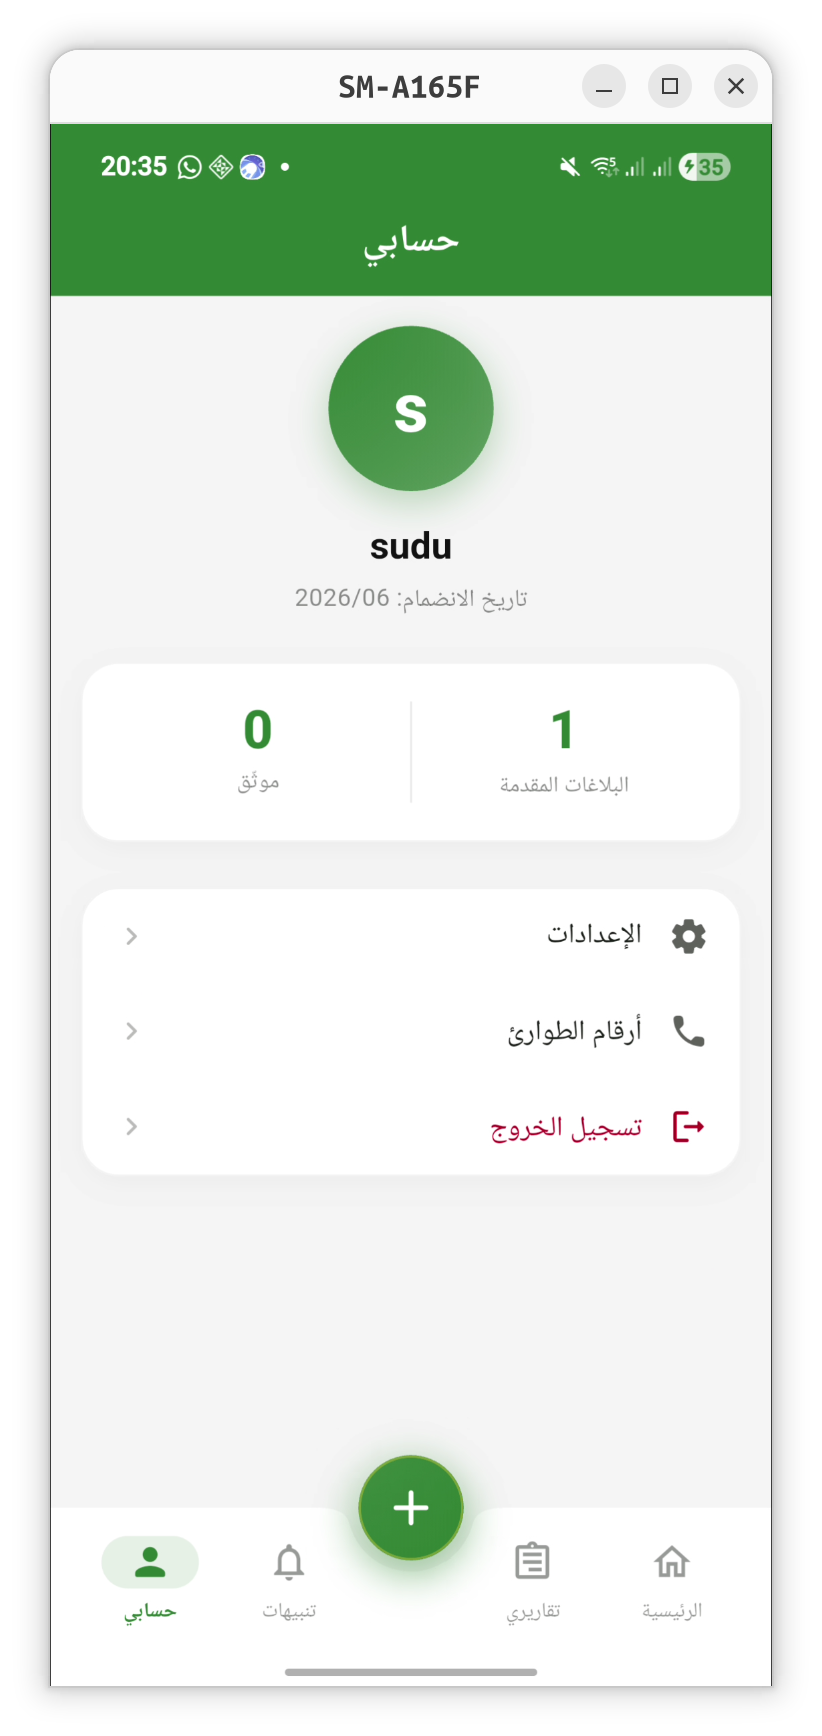
\includegraphics[width=0.4\textwidth]{captures-application/profile.png}
    \caption{Écran de profil utilisateur}
    \label{fig:profile}
\end{figure}

\section{Paramètres}

L'écran des paramètres permet de :
\begin{itemize}
    \item Changer le thème (Clair / Sombre / Système) ;
    \item Changer la langue (Arabe / Français / Anglais) ;
    \item Consulter les informations À propos, Confidentialité et Contact.
\end{itemize}

\begin{figure}[H]
    \centering
    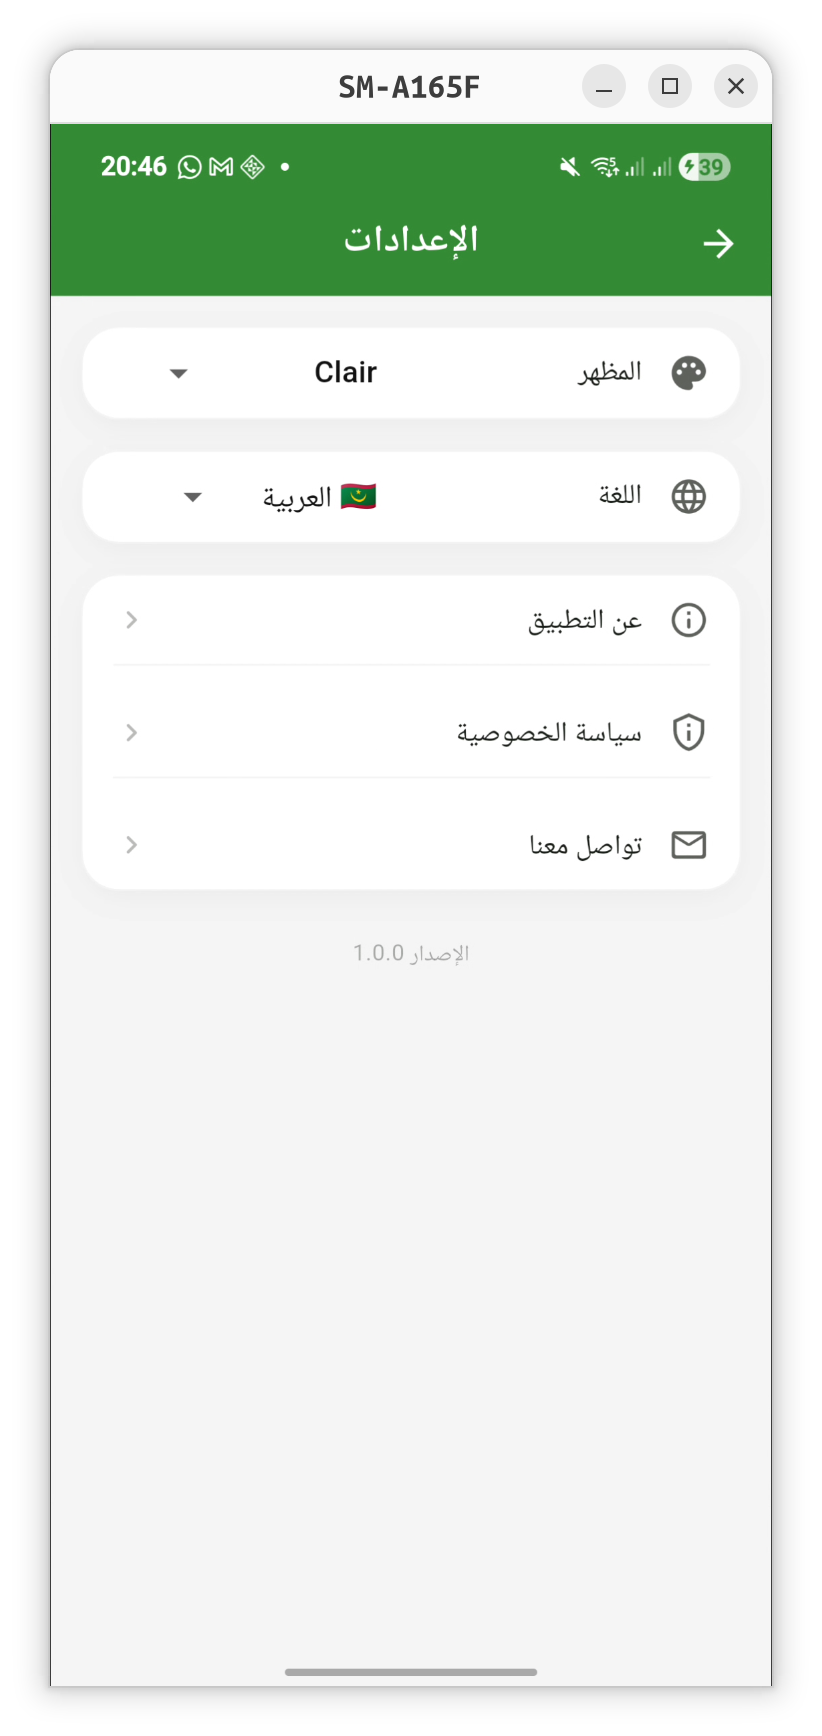
\includegraphics[width=0.4\textwidth]{captures-application/parametre.png}
    \caption{Écran des paramètres}
    \label{fig:parametres}
\end{figure}

\section{Numéros d'urgence}

L'écran des numéros d'urgence (accessible depuis le bouton SOS rouge ou le menu Compte) affiche les contacts essentiels :
\begin{itemize}
    \item \textbf{Pompiers} : 18 ;
    \item \textbf{Ambulance} : 15 ;
    \item \textbf{Hôpital national} : 22 45 25 ;
    \item \textbf{Électricité} : 90 45 23 ;
    \item \textbf{Eau} : 50 45 29 ;
    \item \textbf{Mairie} : 10 45 25 ;
    \item \textbf{SOS Enfants} : 116.
\end{itemize}

Chaque contact dispose d'un bouton d'appel direct.

\begin{figure}[H]
    \centering
    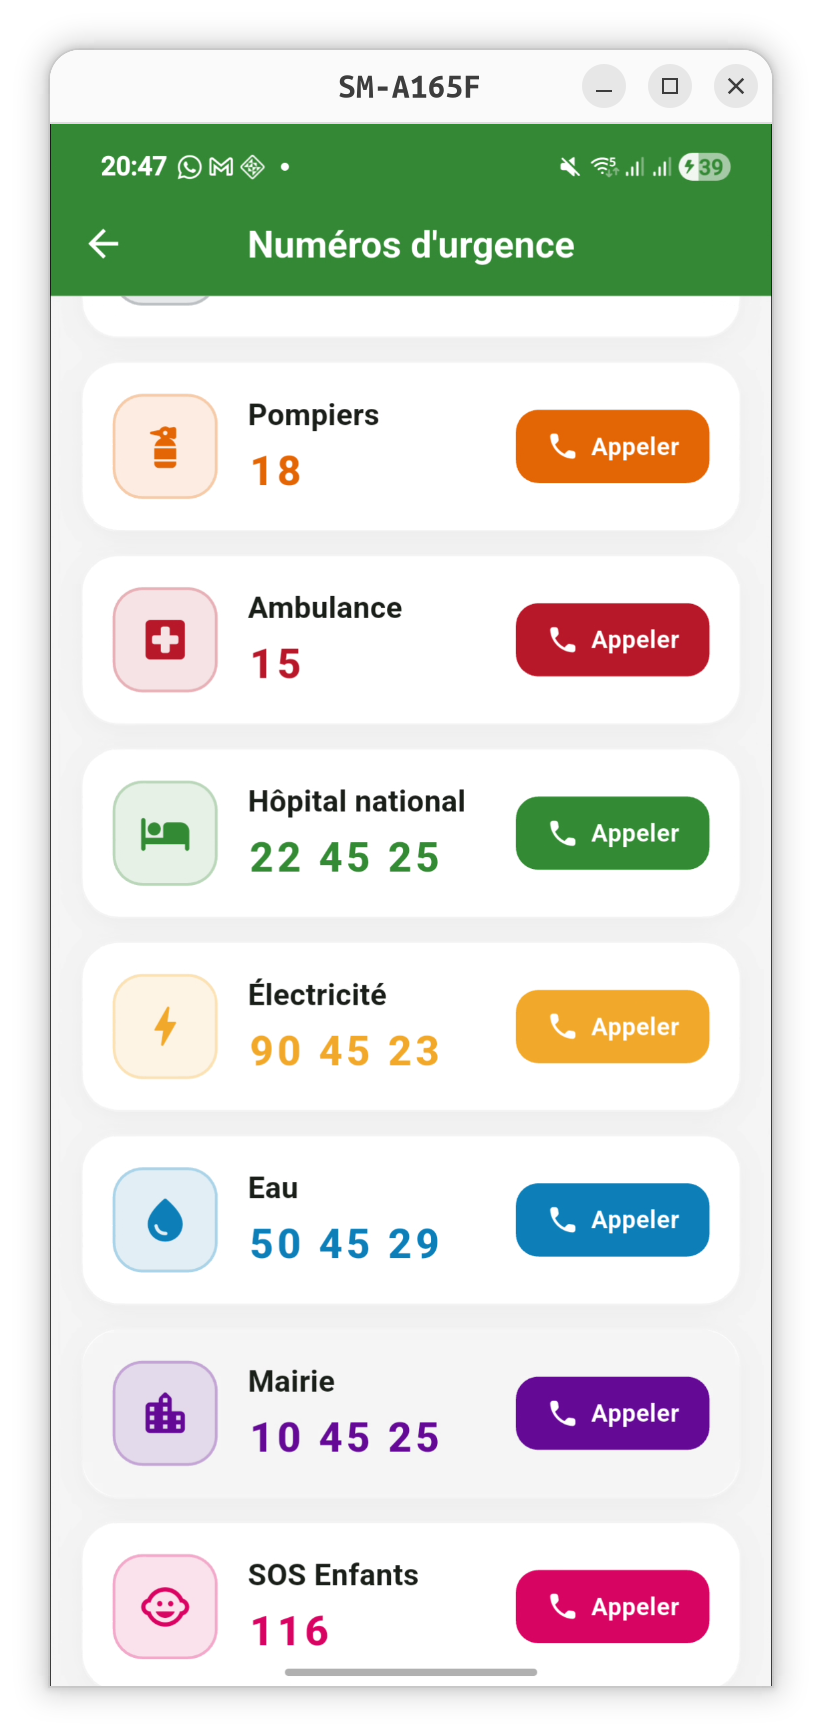
\includegraphics[width=0.4\textwidth]{captures-application/numero_ugence-exeemple.png}
    \caption{Écran des numéros d'urgence}
    \label{fig:urgences}
\end{figure}

\section{Messagerie intégrée}

La messagerie permet aux utilisateurs de communiquer directement à propos d'un signalement :
\begin{itemize}
    \item \textbf{Liste des conversations} : regroupées par (signalement, autre utilisateur) avec aperçu du dernier message et badge non lu ;
    \item \textbf{Chat temps réel} : bulles de messages (envoyé/reçu), horodatage, défilement automatique ;
    \item \textbf{Marquage automatique} : les messages non lus sont marqués comme lus à l'ouverture de la conversation ;
    \item \textbf{Abonnement Realtime} : les nouveaux messages apparaissent instantanément via Supabase Realtime.
\end{itemize}

L'accès à la messagerie se fait depuis l'écran de détail d'un signalement (icône chat dans l'AppBar). Pour un non-auteur, cela ouvre une conversation directe avec l'auteur. Pour l'auteur, cela affiche la liste des conversations liées à ce signalement.

\begin{figure}[H]
    \centering
    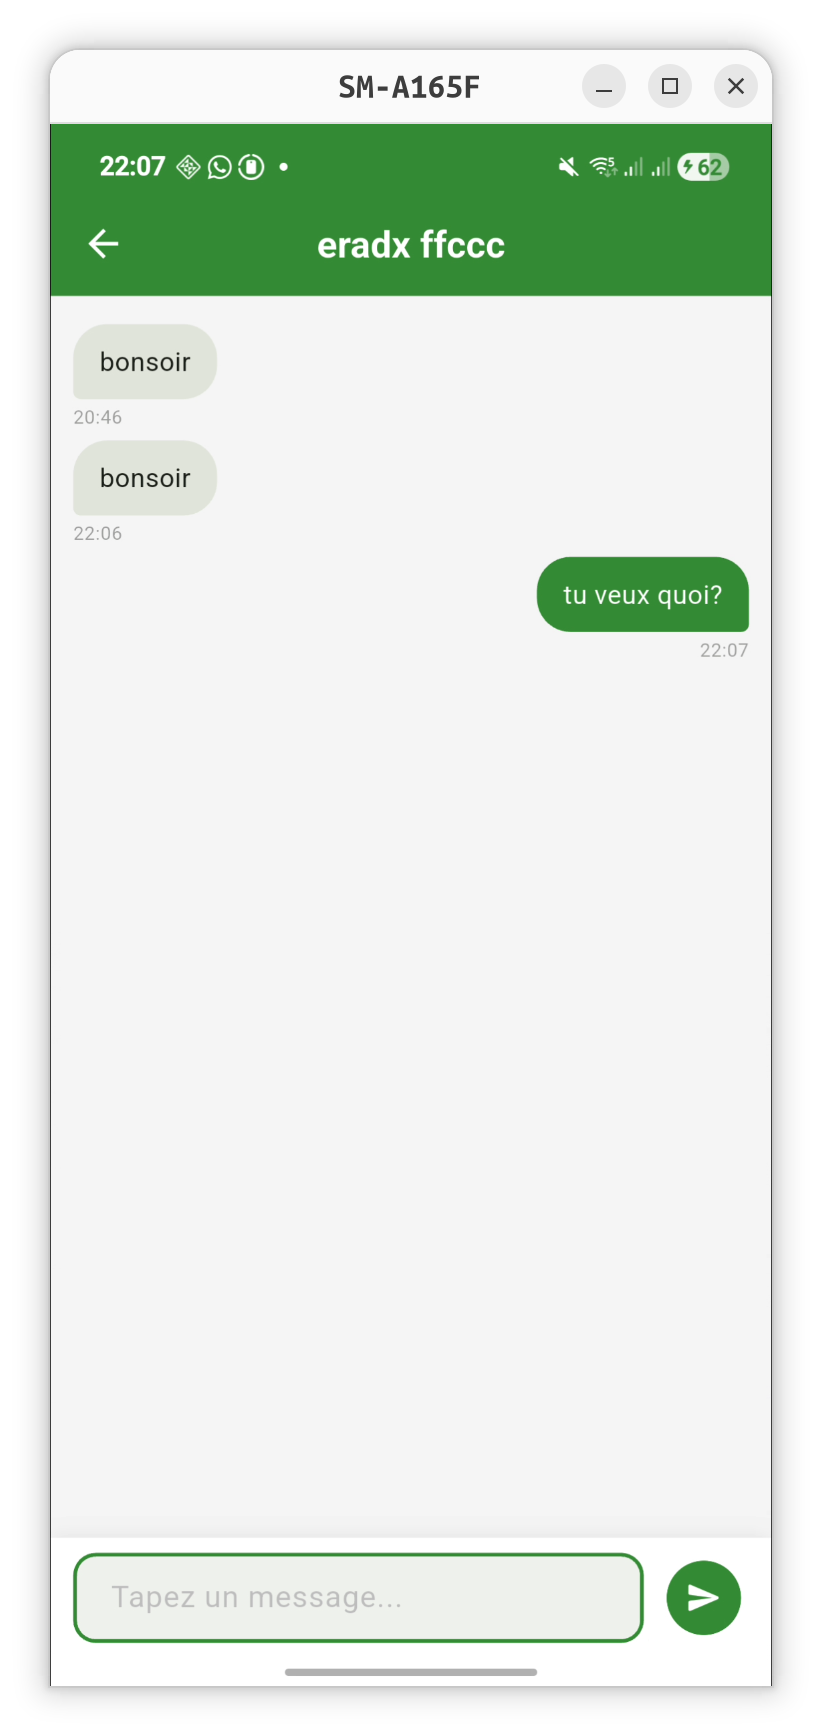
\includegraphics[width=0.4\textwidth]{captures-application/messagerie.png}
    \caption{Interface de messagerie intégrée}
    \label{fig:messagerie}
\end{figure}

\section{Système de vote de crédibilité}

Chaque signalement dispose d'un système de vote :
\begin{itemize}
    \item Bouton \textbf{Confirmer} (crédibilité positive) ;
    \item Bouton \textbf{Infirmer} (crédibilité négative) ;
    \item Barre de progression affichant le pourcentage de crédibilité ;
    \item Un seul vote par utilisateur par signalement (contrainte UNIQUE en base) ;
    \item Mise à jour en temps réel des compteurs via fonction RPC \texttt{update\_vote\_counts}.
\end{itemize}

\section{Tableau de bord d'administration (Web)}

Un tableau de bord web autonome a été développé (HTML/CSS/JS) et déployé sur Vercel. Il permet aux administrateurs de :
\begin{itemize}
    \item Se connecter via Supabase Auth ;
    \item Visualiser et gérer tous les signalements (filtrer, changer le statut, supprimer) ;
    \item Voir la liste des utilisateurs avec statistiques ;
    \item Activer/désactiver le rôle admin ;
    \item Consulter les notifications ;
    \item Graphique des signalements par catégorie (Chart.js).
\end{itemize}

Le dashboard est entièrement internationalisé (arabe/français) avec support RTL/LTR.

\begin{figure}[H]
    \centering
    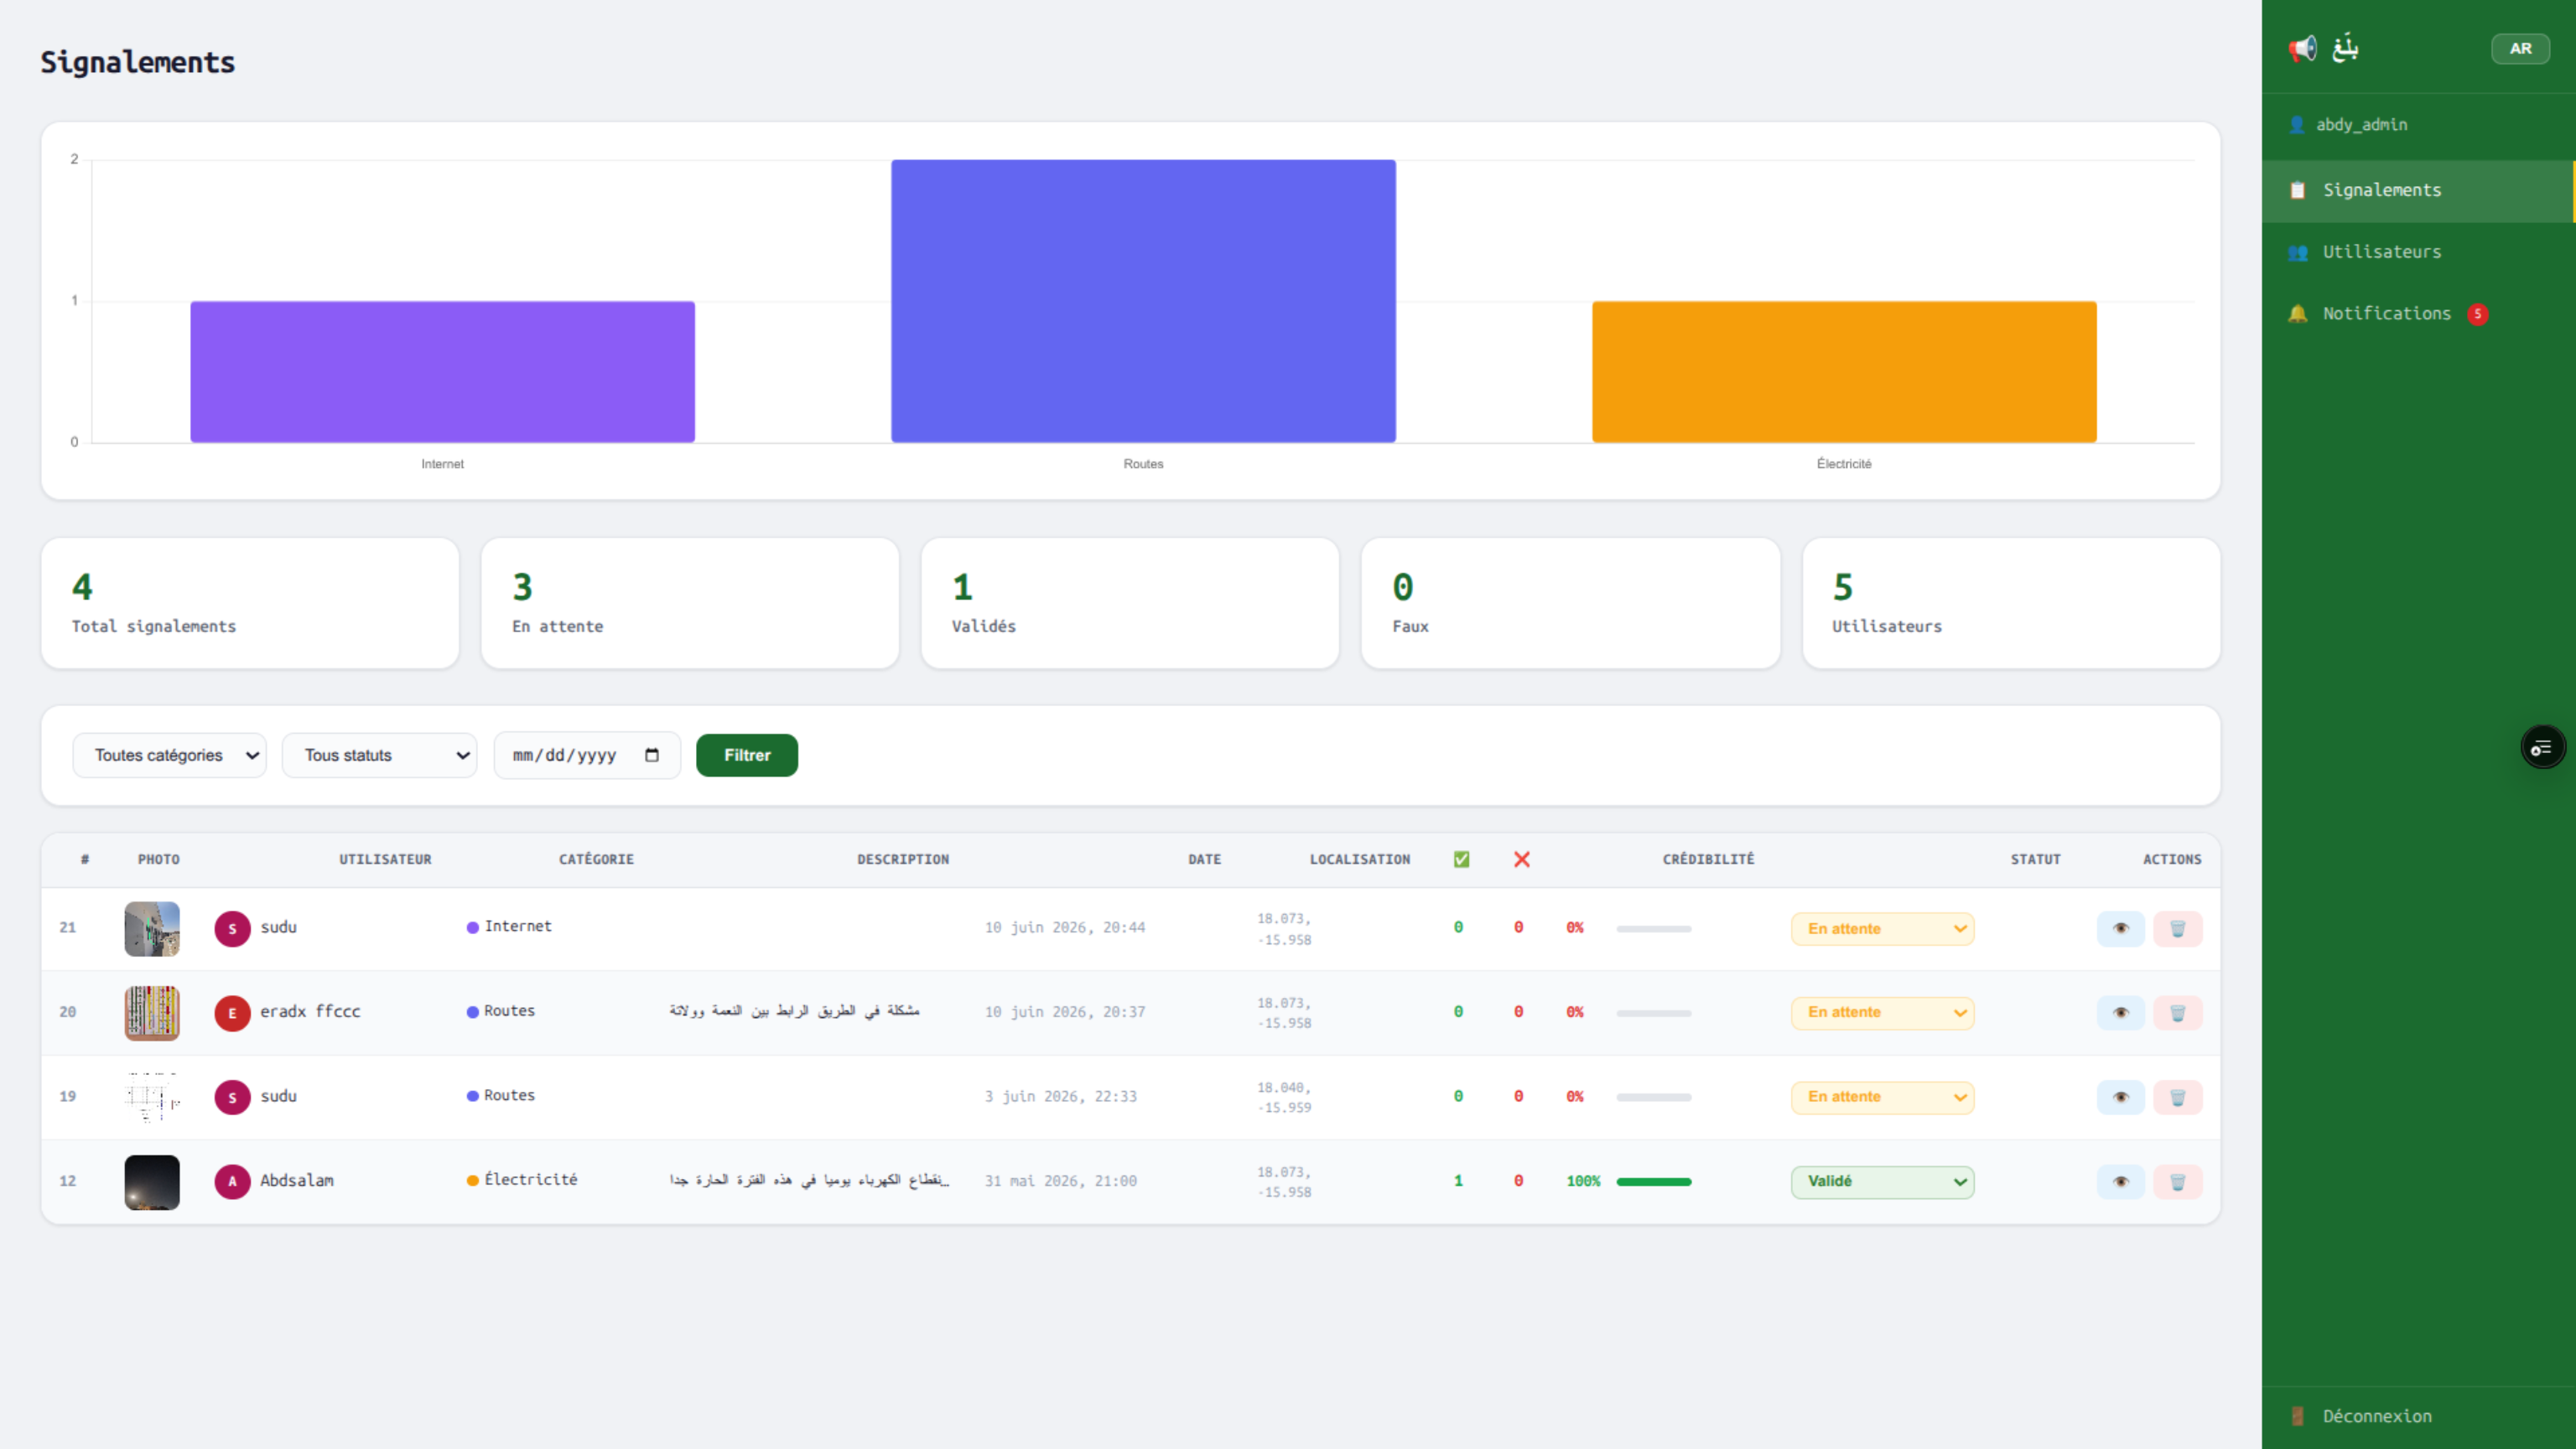
\includegraphics[width=0.8\textwidth]{captures-application/admin-dashboard.png}
    \caption{Tableau de bord d'administration (Web)}
    \label{fig:admin-dashboard}
\end{figure}

\section{Détail des providers (Contrôleurs)}

L'application utilise 9 contrôleurs de type \texttt{ChangeNotifier}, répartis en providers globaux et scopés :

{\small
\begin{longtable}{|p{2.8cm}|p{2.2cm}|p{9.5cm}|}
    \caption{Providers de l'application}
    \label{tab:providers}\\
    \hline
    \rowcolor{supnumgreen!20}
    \textbf{Provider} & \textbf{Portée} & \textbf{Rôle} \\
    \hline
    \endhead
    \hline
    \endfoot
    AuthProvider & Globale & Auth, session persistante \\
    \hline
    ReportProvider & Globale & Liste signalements, CRUD, filtres, votes \\
    \hline
    NavigationProvider & Globale & Onglet actif, navigation 4 écrans \\
    \hline
    ThemeProvider & Globale & Thème clair/sombre, persistance \\
    \hline
    LocaleProvider & Globale & Langue active, persistance \\
    \hline
    AlertProvider & Globale & Notifications DB, compteur non lues \\
    \hline
    ChatProvider & Globale & Messages, conversations, Realtime \\
    \hline
    MapProvider & Scopée & Caméra, marqueurs, sélection, filtres \\
    \hline
    AddReportProvider & Scopée & Wizard 4 étapes, validation, soumission \\
    \hline
\end{longtable}
}

\subsection{Exemple : ReportProvider}

Le \texttt{ReportProvider} est le cœur de l'application. Il gère l'ensemble des signalements :

\begin{lstlisting}[style=codeblock, caption=Extrait de ReportProvider]
class ReportProvider extends ChangeNotifier {
  final ReportServiceDb _reportService;
  List<ReportModel> _allReports = [];
  ReportCategory? _categoryFilter;
  String _searchQuery = '';
  bool _isLoading = false;
  String? _errorMessage;

  List<ReportModel> get filteredReports {
    var reports = _allReports;
    if (_categoryFilter != null) {
      reports = reports
          .where((r) => r.category == _categoryFilter)
          .toList();
    }
    if (_searchQuery.isNotEmpty) {
      final query = _searchQuery.toLowerCase();
      reports = reports.where((r) =>
        r.description.toLowerCase().contains(query) ||
        r.address.toLowerCase().contains(query)
      ).toList();
    }
    return reports;
  }

  Future<void> fetchReports() async {
    _isLoading = true;
    _errorMessage = null;
    notifyListeners();
    try {
      _allReports = await _reportService.getAllReports();
    } catch (e) {
      _errorMessage = e.toString();
    } finally {
      _isLoading = false;
      notifyListeners();
    }
  }

  Future<void> updateCredibility(
    int reportId, String voteType, String userId
  ) async {
    // Appel a vote_dao + RPC update_vote_counts
    // Mise a jour locale immediate
    // notifyListeners()
  }
}
\end{lstlisting}

\subsection{Exemple : AuthProvider}

Le \texttt{AuthProvider} gère l'authentification et la persistance de session :

\begin{lstlisting}[style=codeblock, caption=Extrait d'AuthProvider]
class AuthProvider extends ChangeNotifier {
  final AuthService _authService;
  UserModel? _currentUser;
  bool _isLoading = false;
  bool _isLoggedIn = false;

  UserModel? get currentUser => _currentUser;
  bool get isLoggedIn => _isLoggedIn;

  Future<void> tryAutoLogin() async {
    final session = _authService.currentSession;
    if (session != null) {
      _currentUser = await _authService.getUser(session.user.id);
      _isLoggedIn = true;
      notifyListeners();
    }
  }

  Future<String?> login(String email, String password) async {
    _isLoading = true;
    notifyListeners();
    try {
      final user = await _authService.signIn(email, password);
      _currentUser = user;
      _isLoggedIn = true;
      return null; // succes
    } catch (e) {
      return e.toString(); // message d'erreur
    } finally {
      _isLoading = false;
      notifyListeners();
    }
  }

  Future<void> logout() async {
    await _authService.signOut();
    _currentUser = null;
    _isLoggedIn = false;
    notifyListeners();
  }
}
\end{lstlisting}

\subsection{Exemple : ChatProvider et Realtime}

Le \texttt{ChatProvider} utilise Supabase Realtime pour la messagerie en temps réel :

\begin{lstlisting}[style=codeblock, caption=Extrait de ChatProvider]
class ChatProvider extends ChangeNotifier {
  final MessageDao _messageDao;
  List<Conversation> _conversations = [];
  List<MessageModel> _messages = [];
  int _unreadCount = 0;
  RealtimeChannel? _channel;

  void subscribe(String userId) {
    _channel = supabase.channel('messages:$userId')
      .onPostgresChanges(
        event: PostgresChangeEvent.insert,
        table: 'messages',
        filter: PostgresChangeFilter(
          type: PostgresChangeFilterType.eq,
          column: 'receiver_id',
          value: userId,
        ),
        callback: (payload) {
          _unreadCount++;
          notifyListeners();
        },
      ).subscribe();
  }

  Future<void> sendMessage({
    required int reportId,
    required String senderId,
    required String receiverId,
    required String content,
  }) async {
    final message = MessageModel(
      reportId: reportId,
      senderId: senderId,
      receiverId: receiverId,
      content: content,
    );
    await _messageDao.insert(message);
    // Le callback Realtime mettra a jour l'UI
  }
}
\end{lstlisting}

\subsection{Exemple : AddReportProvider (Wizard)}

Le \texttt{AddReportProvider} gère l'état du formulaire de création en 4 étapes :

\begin{lstlisting}[style=codeblock, caption=Extrait d'AddReportProvider]
class AddReportProvider extends ChangeNotifier {
  int _currentStepIndex = 0;
  ReportCategory? _selectedCategory;
  String _description = '';
  ReportLocation? _location;
  String? _photoUrl;
  bool _isSubmitting = false;

  int get currentStepIndex => _currentStepIndex;
  bool get hasCategory => _selectedCategory != null;
  bool get isLastStep => _currentStepIndex == 3;

  void selectCategory(ReportCategory category) {
    _selectedCategory = category;
    notifyListeners();
  }

  void setDescription(String text) {
    _description = text;
    // Pas de notifyListeners() pour eviter les rebuilds inutiles
  }

  void setLocation(ReportLocation location) {
    _location = location;
    notifyListeners();
  }

  void nextStep() {
    if (_currentStepIndex < 3) _currentStepIndex++;
    notifyListeners();
  }

  Map<String, dynamic> buildDraft() {
    return {
      'category': _selectedCategory?.name,
      'description': _description,
      'latitude': _location?.latitude,
      'longitude': _location?.longitude,
      'address': _location?.address,
      'photo_url': _photoUrl,
    };
  }
}
\end{lstlisting}

\section{Support multilingue}

L'application supporte trois langues :
\begin{itemize}
    \item \textbf{Arabe} (\texttt{ar}) -- écriture RTL, police Cairo ;
    \item \textbf{Français} (\texttt{fr}) -- écriture LTR ;
    \item \textbf{Anglais} (\texttt{en}) -- écriture LTR.
\end{itemize}

Plus de 95 clés de traduction sont implémentées, couvrant tous les écrans et composants. Le changement de langue est instantané et persisté.

\section{Thèmes (Clair / Sombre)}

L'application utilise \textbf{Material 3} avec deux thèmes complets :
\begin{itemize}
    \item \textbf{Thème clair} : fond blanc, vert brand (\#2E7D32), jaune (\#FDD835) ;
    \item \textbf{Thème sombre} : fond foncé, mêmes couleurs d'accentuation adaptées ;
    \item \textbf{Mode système} : suit automatiquement les préférences du système.
\end{itemize}

Le choix du thème est persisté via \texttt{SharedPreferences}.

\section{Environnement de développement}

Le projet a été développé et testé dans l'environnement suivant :

{\small
\begin{table}[H]
    \centering
    \begin{tabular}{|l|l|}
        \hline
        \rowcolor{supnumgreen!20}
        \textbf{Composant} & \textbf{Version / Spécification} \\
        \hline
        Système d'exploitation & Ubuntu 22.04 LTS \\
        \hline
        Flutter & 3.3+ (Dart 3.x) \\
        \hline
        Langage & Dart 3.3+ \\
        \hline
        IDE & VS Code + Android Studio \\
        \hline
        SDK Android & API 23+ (Android 7.0) \\
        \hline
        Gestion d'état & Provider 6.1.2 \\
        \hline
        Backend & Supabase (PostgreSQL 15) \\
        \hline
        Cartographie & flutter\_map + FMTC \\
        \hline
        Géolocalisation & geolocator 13.0.1 \\
        \hline
        Stockage photos & Supabase Storage \\
        \hline
        Authentification & Supabase Auth + Google OAuth \\
        \hline
        Internationalisation & intl + flutter\_localizations \\
        \hline
        Déploiement admin & Vercel \\
        \hline
        Gestion de versions & Git + GitHub \\
        \hline
    \end{tabular}
    \caption{Environnement de développement}
    \label{tab:dev-env}
\end{table}
}

\section{Tableau récapitulatif des fonctionnalités}

{\small
\begin{longtable}{|p{3cm}|p{4cm}|p{2.5cm}|p{4.5cm}|}
    \caption{Récapitulatif des fonctionnalités développées}
    \label{tab:features}\\
    \hline
    \rowcolor{supnumgreen!20}
    \textbf{Fonctionnalité} & \textbf{Composant} & \textbf{Statut} & \textbf{Technologie} \\
    \hline
    \endhead
    \hline
    \endfoot
    Authentification & AuthProvider + AuthService & \done{}  Fait & Supabase Auth \\
    \hline
    Création signalement & Wizard 4 étapes & \done{}  Fait & Flutter + Supabase \\
    \hline
    Liste signalements & HomeView + ReportProvider & \done{}  Fait & Flutter + Supabase \\
    \hline
    Carte interactive & MapView + MapProvider & \done{}  Fait & flutter\_map + OSM \\
    \hline
    Détail + Votes & ReportDetailView & \done{}  Fait & Flutter + Supabase \\
    \hline
    Mes signalements & MyReportsView & \done{}  Fait & Flutter + Supabase \\
    \hline
    Notifications & AlertProvider + AlertView & \done{}  Fait & Supabase Realtime \\
    \hline
    Messagerie & ChatProvider + ChatView & \done{}  Fait & Supabase Realtime \\
    \hline
    Internationalisation & L10n + ARB files & \done{}  Fait & intl + ARB \\
    \hline
    Thème clair/sombre & ThemeProvider & \done{}  Fait & Material 3 \\
    \hline
    Profil utilisateur & AccountView & \done{}  Fait & Flutter + Supabase \\
    \hline
    Paramètres & SettingsView & \done{}  Fait & Flutter \\
    \hline
    Numéros urgence & EmergencyNumbersView & \done{}  Fait & url\_launcher \\
    \hline
    Dashboard admin & Admin (Web) & \done{}  Fait & HTML/CSS/JS + Supabase \\
    \hline
    Photos & Step 3 + Supabase Storage & \done{}  Fait & image\_picker \\
    \hline
\end{longtable}
}

% =====================================================
% CHAPITRE 6 : CONCLUSION
% =====================================================
\chapter{Conclusion}

\section{Respect du cahier des charges}

Le projet Baligh respecte l'ensemble des consignes administratives du module de Développement Mobile :

{\small
\begin{longtable}{|p{4.5cm}|p{2.5cm}|p{6.5cm}|}
    \caption{Respect des consignes administratives}
    \label{tab:consignes}\\
    \hline
    \rowcolor{supnumgreen!20}
    \textbf{Consigne} & \textbf{Statut} & \textbf{Justification} \\
    \hline
    \endhead
    \hline
    \endfoot
    Travail en groupe (4 étudiants) & \done{}  Respecté & 4 membres, répartition des tâches \\
    \hline
    Fonctionnalités interactives & \done{}  Respecté & Formulaires, navigation, CRUD \\
    \hline
    Gestion d'état (Provider) & \done{}  Respecté & 9 ChangeNotifier providers \\
    \hline
    Architecture MVC & \done{}  Respecté & Models / Views / Controllers / Services \\
    \hline
    Base de données & \done{}  Respecté & Supabase PostgreSQL avec RLS \\
    \hline
    API & \done{}  Respecté & Supabase REST + Realtime + Storage \\
    \hline
    Internationalisation (2+ langues) & \done{}  Respecté & 3 langues : français, anglais, arabe \\
    \hline
    Code clair et structuré & \done{}  Respecté & Organisation logique, conventions Flutter \\
    \hline
    Présentation finale & \done{}  Préparé & Rapport + soutenance \\
    \hline
    Originalité du projet & \done{}  Validé & Application citoyenne adaptée à la Mauritanie \\
    \hline
\end{longtable}
}

\section{Bilan du projet}

Le projet \textbf{Baligh} a permis de développer une application mobile complète de signalement citoyen, répondant aux objectifs fixés par le cahier des charges du module de Développement Mobile de SUPNUM.

L'ensemble des fonctionnalités demandées a été implémenté :
\begin{itemize}
    \item Application interactive avec formulaires, navigation multi-écrans et CRUD complet ;
    \item Gestion d'état avec \textbf{Provider} (9 contrôleurs ChangeNotifier) ;
    \item Architecture \textbf{MVC} avec séparation claire des couches (Modèles, Vues, Contrôleurs, Services, DAOs) ;
    \item Connexion à une \textbf{base de données distante} (Supabase PostgreSQL) et à une \textbf{API} (Supabase REST, Realtime, Storage) ;
    \item \textbf{Internationalisation} complète (arabe, français, anglais) avec plus de 95 clés de traduction ;
    \item Code structuré et maintenable (organisation logique des fichiers, bonnes pratiques).
\end{itemize}

\section{Difficultés rencontrées}

Plusieurs difficultés ont été rencontrées et résolues au cours du projet :

\begin{enumerate}
    \item \textbf{Gestion d'état complexe} : coordination entre plusieurs providers (Auth, Report, Map, Chat) nécessitant une conception minutieuse des dépendances ;
    \item \textbf{Cartographie} : configuration de flutter\_map avec FMTC, optimisation des marqueurs pour éviter les rebuilds excessifs ;
    \item \textbf{Sécurité RLS} : configuration des politiques Row Level Security pour les votes et notifications (contournement via fonctions SECURITY DEFINER) ;
    \item \textbf{Google Sign-In} : résolution des problèmes de configuration (SHA-1, clientId, serverClientId) ;
    \item \textbf{Photos} : intégration de l'upload vers Supabase Storage avec gestion des permissions ;
    \item \textbf{Temps réel} : implémentation des subscriptions Realtime pour la messagerie et les notifications.
\end{enumerate}

\section{Compétences acquises}

Ce projet a permis aux membres de l'équipe d'acquérir et de consolider les compétences suivantes :

\begin{itemize}
    \item \textbf{Développement Flutter} : widgets, états, navigation, animations ;
    \item \textbf{Gestion d'état} : Provider, ChangeNotifier, Selector, Consumer ;
    \item \textbf{Backend mobile} : Supabase (Auth, Database, Storage, Realtime) ;
    \item \textbf{Cartographie} : flutter\_map, OpenStreetMap, FMTC, géocodage ;
    \item \textbf{Internationalisation} : ARB files, flutter\_localizations, support RTL ;
    \item \textbf{Sécurité} : RLS (Row Level Security), JWT, OAuth 2.0 ;
    \item \textbf{Travail en équipe} : Git, GitHub, méthodologie agile, répartition des tâches.
\end{itemize}

\section{Calendrier du projet}

Le projet s'est déroulé sur un semestre (environ 16 semaines), selon le calendrier suivant :

\begin{table}[H]
    \centering
    \begin{tabular}{|c|l|l|}
        \hline
        \rowcolor{supnumgreen!20}
        \textbf{Période} & \textbf{Activités} & \textbf{Livrables} \\
        \hline
        Semaines 1--2 & Analyse des besoins, conception & Cahier des charges, maquettes \\
        \hline
        Semaines 3--4 & Mise en place environnement, Flutter & Projet de base, dépôt Git \\
        \hline
        Semaines 5--6 & Authentification, base Supabase & Auth, DAOs, écrans login/register \\
        \hline
        Semaines 7--8 & Écran d'accueil, liste signalements & HomeView, ReportCard, Provider \\
        \hline
        Semaines 9--10 & Cartographie, assistant signalement & MapView, AddReport wizard (4 étapes) \\
        \hline
        Semaines 11--12 & Votes, messagerie, notifications & Vote system, Chat, Notifications \\
        \hline
        Semaines 13--14 & Internationalisation, thèmes, admin & ARB 3 langues, dashboard web \\
        \hline
        Semaines 15--16 & Tests, déploiement, documentation & APK, déploiement Vercel, rapport \\
        \hline
    \end{tabular}
    \caption{Calendrier de réalisation du projet}
    \label{tab:calendar}
\end{table}

\section{Perspectives d'amélioration}

Le projet pourrait être amélioré dans les directions suivantes :

\begin{itemize}
    \item \textbf{Performance} : optimisation des rebuilds dans la carte (Selectors granulaires, memoization des marqueurs) ;
    \item \textbf{Fonctionnalités sociales} : commentaires, likes, partage sur les réseaux sociaux ;
    \item \textbf{Notifications push} : intégration de Firebase Cloud Messaging (FCM) ;
    \item \textbf{Mode hors ligne} : synchronisation des signalements en l'absence de connexion ;
    \item \textbf{Analytics} : tableau de bord des tendances par région, catégorie, période ;
    \item \textbf{Version web} : déploiement Flutter Web complet (au-delà du dashboard admin).
\end{itemize}

\section{Conclusion finale}

Le projet \textbf{Baligh} constitue une solution innovante et adaptée au contexte mauritanien pour le signalement citoyen. Il démontre la capacité de l'équipe à concevoir, développer et déployer une application mobile complète en utilisant les technologies modernes du développement mobile (Flutter, Dart, Supabase).

En respectant l'ensemble des contraintes du cahier des charges (MVC, Provider, base de données, API, internationalisation, code structuré), ce projet atteint les objectifs pédagogiques fixés et constitue une base solide pour un déploiement à plus grande échelle.

\begin{center}
    \vspace{1cm}
    \textbf{« Parce que chaque voix compte. »} \\
    \textit{Baligh --- Because every voice matters.}
    \vspace{1cm}
\end{center}

% =====================================================
% BIBLIOGRAPHIE
% =====================================================
\chapter*{Bibliographie}
\addcontentsline{toc}{chapter}{Bibliographie}
\begin{thebibliography}{99}

\bibitem{flutter-docs}
Flutter Documentation. \textit{Flutter.dev}. Google.
\url{https://docs.flutter.dev}

\bibitem{dart-docs}
Dart Programming Language. \textit{Dart.dev}. Google.
\url{https://dart.dev}

\bibitem{provider-package}
Provider Package. \textit{Pub.dev}. Flutter.
\url{https://pub.dev/packages/provider}

\bibitem{supabase-docs}
Supabase Documentation. \textit{Supabase.com}.
\url{https://supabase.com/docs}

\bibitem{flutter-map}
flutter\_map Package. \textit{Pub.dev}.
\url{https://pub.dev/packages/flutter_map}

\bibitem{flutter-map-tile-caching}
flutter\_map\_tile\_caching Package. \textit{Pub.dev}.
\url{https://pub.dev/packages/flutter_map_tile_caching}

\bibitem{openstreetmap}
OpenStreetMap. \textit{OpenStreetMap.org}.
\url{https://www.openstreetmap.org}

\bibitem{google-fonts}
Google Fonts -- Cairo. \textit{Google Fonts}.
\url{https://fonts.google.com/specimen/Cairo}

\bibitem{flutter-i18n}
Internationalization (Flutter). \textit{Flutter.dev}.
\url{https://docs.flutter.dev/ui/accessibility-and-localization/internationalization}

\bibitem{material3}
Material Design 3. \textit{Material.io}. Google.
\url{https://m3.material.io}

\bibitem{supabase-rls}
Row Level Security (Supabase). \textit{Supabase.com}.
\url{https://supabase.com/docs/guides/auth/row-level-security}

\bibitem{supabase-realtime}
Realtime (Supabase). \textit{Supabase.com}.
\url{https://supabase.com/docs/guides/realtime}

\bibitem{geolocator}
geolocator Package. \textit{Pub.dev}.
\url{https://pub.dev/packages/geolocator}

\bibitem{image-picker}
image\_picker Package. \textit{Pub.dev}.
\url{https://pub.dev/packages/image_picker}

\bibitem{share-plus}
share\_plus Package. \textit{Pub.dev}.
\url{https://pub.dev/packages/share_plus}

\bibitem{url-launcher}
url\_launcher Package. \textit{Pub.dev}.
\url{https://pub.dev/packages/url_launcher}

\bibitem{google-signin}
google\_sign\_in Package. \textit{Pub.dev}.
\url{https://pub.dev/packages/google_sign_in}

\bibitem{chartjs}
Chart.js. \textit{Chartjs.org}.
\url{https://www.chartjs.org}

\bibitem{vercel}
Vercel Documentation. \textit{Vercel.com}.
\url{https://vercel.com/docs}

\bibitem{flutter-themes}
Themes (Flutter). \textit{Flutter.dev}.
\url{https://docs.flutter.dev/ui/design/material}

\end{thebibliography}

\end{document}
